%% Beginning of file 'sample631.tex'
%%
%% Modified 2021 March
%%
%% This is a sample manuscript marked up using the
%% AASTeX v6.31 LaTeX 2e macros.
%%
%% AASTeX is now based on Alexey Vikhlinin's emulateapj.cls 
%% (Copyright 2000-2015).  See the classfile for details.

%% AASTeX requires revtex4-1.cls and other external packages such as
%% latexsym, graphicx, amssymb, longtable, and epsf.  Note that as of 
%% Oct 2020, APS now uses revtex4.2e for its journals but remember that 
%% AASTeX v6+ still uses v4.1. All of these external packages should 
%% already be present in the modern TeX distributions but not always.
%% For example, revtex4.1 seems to be missing in the linux version of
%% TexLive 2020. One should be able to get all packages from www.ctan.org.
%% In particular, revtex v4.1 can be found at 
%% https://www.ctan.org/pkg/revtex4-1.

%% The first piece of markup in an AASTeX v6.x document is the \documentclass
%% command. LaTeX will ignore any data that comes before this command. The 
%% documentclass can take an optional argument to modify the output style.
%% The command below calls the preprint style which will produce a tightly 
%% typeset, one-column, single-spaced document.  It is the default and thus
%% does not need to be explicitly stated.
%%
%% using aastex version 6.3
\documentclass[linenumbers, twocolumn]{aastex631}

%% The default is a single spaced, 10 point font, single spaced article.
%% There are 5 other style options available via an optional argument. They
%% can be invoked like this:
%%
%% \documentclass[arguments]{aastex631}
%% 
%% where the layout options are:
%%
%%  twocolumn   : two text columns, 10 point font, single spaced article.
%%                This is the most compact and represent the final published
%%                derived PDF copy of the accepted manuscript from the publisher
%%  manuscript  : one text column, 12 point font, double spaced article.
%%  preprint    : one text column, 12 point font, single spaced article.  
%%  preprint2   : two text columns, 12 point font, single spaced article.
%%  modern      : a stylish, single text column, 12 point font, article with
%% 		  wider left and right margins. This uses the Daniel
%% 		  Foreman-Mackey and David Hogg design.
%%  RNAAS       : Supresses an abstract. Originally for RNAAS manuscripts 
%%                but now that abstracts are required this is obsolete for
%%                AAS Journals. Authors might need it for other reasons. DO NOT
%%                use \begin{abstract} and \end{abstract} with this style.
%%
%% Note that you can submit to the AAS Journals in any of these 6 styles.
%%
%% There are other optional arguments one can invoke to allow other stylistic
%% actions. The available options are:
%%
%%   astrosymb    : Loads Astrosymb font and define \astrocommands. 
%%   tighten      : Makes baselineskip slightly smaller, only works with 
%%                  the twocolumn substyle.
%%   times        : uses times font instead of the default
%%   linenumbers  : turn on lineno package.
%%   trackchanges : required to see the revision mark up and print its output
%%   longauthor   : Do not use the more compressed footnote style (default) for 
%%                  the author/collaboration/affiliations. Instead print all
%%                  affiliation information after each name. Creates a much 
%%                  longer author list but may be desirable for short 
%%                  author papers.
%% twocolappendix : make 2 column appendix.
%%   anonymous    : Do not show the authors, affiliations and acknowledgments 
%%                  for dual anonymous review.
%%
%% these can be used in any combination, e.g.
%%
%% \documentclass[twocolumn,linenumbers,trackchanges]{aastex631}
%%
%% AASTeX v6.* now includes \hyperref support. While we have built in specific
%% defaults into the classfile you can manually override them with the
%% \hypersetup command. For example,
%%
%% \hypersetup{linkcolor=red,citecolor=green,filecolor=cyan,urlcolor=magenta}
%%
%% will change the color of the internal links to red, the links to the
%% bibliography to green, the file links to cyan, and the external links to
%% magenta. Additional information on \hyperref options can be found here:
%% https://www.tug.org/applications/hyperref/manual.html#x1-40003
%%
%% Note that in v6.3 "bookmarks" has been changed to "true" in hyperref
%% to improve the accessibility of the compiled pdf file.
%%
%% If you want to create your own macros, you can do so
%% using \newcommand. Your macros should appear before
%% the \begin{document} command.
%%
\newcommand{\vdag}{(v)^\dagger}
\newcommand\aastex{AAS\TeX}
\newcommand\latex{La\TeX}

%% Reintroduced the \received and \accepted commands from AASTeX v5.2
%\received{March 1, 2021}
%\revised{April 1, 2021}
%\accepted{\today}

%% Command to document which AAS Journal the manuscript was submitted to.
%% Adds "Submitted to " the argument.
%\submitjournal{PSJ}

%% For manuscript that include authors in collaborations, AASTeX v6.31
%% builds on the \collaboration command to allow greater freedom to 
%% keep the traditional author+affiliation information but only show
%% subsets. The \collaboration command now must appear AFTER the group
%% of authors in the collaboration and it takes TWO arguments. The last
%% is still the collaboration identifier. The text given in this
%% argument is what will be shown in the manuscript. The first argument
%% is the number of author above the \collaboration command to show with
%% the collaboration text. If there are authors that are not part of any
%% collaboration the \nocollaboration command is used. This command takes
%% one argument which is also the number of authors above to show. A
%% dashed line is shown to indicate no collaboration. This example manuscript
%% shows how these commands work to display specific set of authors 
%% on the front page.
%%
%% For manuscript without any need to use \collaboration the 
%% \AuthorCollaborationLimit command from v6.2 can still be used to 
%% show a subset of authors.
%
%\AuthorCollaborationLimit=2
%
%% will only show Schwarz & Muench on the front page of the manuscript
%% (assuming the \collaboration and \nocollaboration commands are
%% commented out).
%%
%% Note that all of the author will be shown in the published article.
%% This feature is meant to be used prior to acceptance to make the
%% front end of a long author article more manageable. Please do not use
%% this functionality for manuscripts with less than 20 authors. Conversely,
%% please do use this when the number of authors exceeds 40.
%%
%% Use \allauthors at the manuscript end to show the full author list.
%% This command should only be used with \AuthorCollaborationLimit is used.

%% The following command can be used to set the latex table counters.  It
%% is needed in this document because it uses a mix of latex tabular and
%% AASTeX deluxetables.  In general it should not be needed.
%\setcounter{table}{1}

%%%%%%%%%%%%%%%%%%%%%%%%%%%%%%%%%%%%%%%%%%%%%%%%%%%%%%%%%%%%%%%%%%%%%%%%%%%%%%%%
%%
%% The following section outlines numerous optional output that
%% can be displayed in the front matter or as running meta-data.
%%
%% If you wish, you may supply running head information, although
%% this information may be modified by the editorial offices.
\shorttitle{ASPIRED toolkit}
\shortauthors{Lam et al.}
%%
%% You can add a light gray and diagonal water-mark to the first page 
%% with this command:
%% \watermark{text}
%% where "text", e.g. DRAFT, is the text to appear.  If the text is 
%% long you can control the water-mark size with:
%% \setwatermarkfontsize{dimension}
%% where dimension is any recognized LaTeX dimension, e.g. pt, in, etc.
%%
%%%%%%%%%%%%%%%%%%%%%%%%%%%%%%%%%%%%%%%%%%%%%%%%%%%%%%%%%%%%%%%%%%%%%%%%%%%%%%%%
\graphicspath{{./}{figures/}}
%% This is the end of the preamble.  Indicate the beginning of the
%% manuscript itself with \begin{document}.

\begin{document}

\title{Automated SpectroPhotometric Image REDuction (ASPIRED) -- \\ A \textsc{Python}-based spectral data reduction toolkit\\}


%% LaTeX will automatically break titles if they run longer than
%% one line. However, you may use \\ to force a line break if
%% you desire. In v6.31 you can include a footnote in the title.

%% A significant change from earlier AASTEX versions is in the structure for 
%% calling author and affiliations. The change was necessary to implement 
%% auto-indexing of affiliations which prior was a manual process that could 
%% easily be tedious in large author manuscripts.
%%
%% The \author command is the same as before except it now takes an optional
%% argument which is the 16 digit ORCID. The syntax is:
%% \author[xxxx-xxxx-xxxx-xxxx]{Author Name}
%%
%% This will hyperlink the author name to the author's ORCID page. Note that
%% during compilation, LaTeX will do some limited checking of the format of
%% the ID to make sure it is valid. If the "orcid-ID.png" image file is 
%% present or in the LaTeX pathway, the OrcID icon will appear next to
%% the authors name.
%%
%% Use \affiliation for affiliation information. The old \affil is now aliased
%% to \affiliation. AASTeX v6.31 will automatically index these in the header.
%% When a duplicate is found its index will be the same as its previous entry.
%%
%% Note that \altaffilmark and \altaffiltext have been removed and thus 
%% can not be used to document secondary affiliations. If they are used latex
%% will issue a specific error message and quit. Please use multiple 
%% \affiliation calls for to document more than one affiliation.
%%
%% The new \altaffiliation can be used to indicate some secondary information
%% such as fellowships. This command produces a non-numeric footnote that is
%% set away from the numeric \affiliation footnotes.  NOTE that if an
%% \altaffiliation command is used it must come BEFORE the \affiliation call,
%% right after the \author command, in order to place the footnotes in
%% the proper location.
%%
%% Use \email to set provide email addresses. Each \email will appear on its
%% own line so you can put multiple email address in one \email call. A new
%% \correspondingauthor command is available in V6.31 to identify the
%% corresponding author of the manuscript. It is the author's responsibility
%% to make sure this name is also in the author list.
%%
%% While authors can be grouped inside the same \author and \affiliation
%% commands it is better to have a single author for each. This allows for
%% one to exploit all the new benefits and should make book-keeping easier.
%%
%% If done correctly the peer review system will be able to
%% automatically put the author and affiliation information from the manuscript
%% and save the corresponding author the trouble of entering it by hand.

%\correspondingauthor{August Muench}
%\email{greg.schwarz@aas.org, gus.muench@aas.org}

\author[0000-0002-9347-2298]{Marco C. Lam}
\affiliation{School of Physics and Astronomy, Tel Aviv University, Tel Aviv 69978, Israel
}
\affiliation{Astrophysics Research Institute, Liverpool John Moores University, IC2, LSP, 146 Brownlow Hill, Liverpool L3 5RF, UK}
\affiliation{Astronomical Observatory, University of Warsaw, Al. Ujazdowskie 4, 00-478, Warszawa, Poland}

\author[0000-0003-3434-1922]{Robert J. Smith}
\affiliation{Astrophysics Research Institute, Liverpool John Moores University, IC2, LSP, 146 Brownlow Hill, Liverpool L3 5RF, UK}

\author[0000-0001-7090-4898]{Iair Arcavi}
\affiliation{School of Physics and Astronomy, Tel Aviv University, Tel Aviv 69978, Israel}
\affiliation{CIFAR Azrieli Global Scholars program, CIFAR, Toronto, Canada}

\author[0000-0001-8397-5759]{Iain A. Steele}
\affiliation{Astrophysics Research Institute, Liverpool John Moores University, IC2, LSP, 146 Brownlow Hill, Liverpool L3 5RF, UK}

\author[0000-0003-2780-7843]{Josh Veitch-Michaelis}
\affiliation{Astrophysics Research Institute, Liverpool John Moores University, IC2, LSP, 146 Brownlow Hill, Liverpool L3 5RF, UK}
\affiliation{Department of Physics and Wisconsin IceCube Particle Astrophysics Center, University of Wisconsin, Madison, WI 53706, USA}
\affiliation{ETH Z\"urich, Systems Group, Stampfenbachstrasse 114, 8092 Z\"urich, Switzerland}

\author[0000-0002-9658-6151]{Lukasz Wyrzykowski}
\affiliation{Astronomical Observatory, University of Warsaw, Al. Ujazdowskie 4, 00-478, Warszawa, Poland}


%% Note that the \and command from previous versions of AASTeX is now
%% depreciated in this version as it is no longer necessary. AASTeX 
%% automatically takes care of all commas and "and"s between authors names.

%% AASTeX 6.31 has the new \collaboration and \nocollaboration commands to
%% provide the collaboration status of a group of authors. These commands 
%% can be used either before or after the list of corresponding authors. The
%% argument for \collaboration is the collaboration identifier. Authors are
%% encouraged to surround collaboration identifiers with ()s. The 
%% \nocollaboration command takes no argument and exists to indicate that
%% the nearby authors are not part of surrounding collaborations.

%% Mark off the abstract in the ``abstract'' environment. 
\begin{abstract}
%%%%%%%%%%%%%%%%%%%%%%%%%%%%%%%%%%%%%%%%%%%%%%%%%%%%%%%%%%%%%%%%%%%%%%%%%%%%%%%%
We provide a suite of open-source spectral data reduction software publicly
available for all interested users, to facilitate rapid scientific products
from all forms of long-slit-like spectroscopic observations. The Automated
SpectroPhotometric REDuction (\textsc{ASPIRED}) toolkit is designed to be a
general toolkit with high flexibility for users to refine and tailor-make
their data reduction routines optimised for the individual characteristics
of their instruments. The default configuration is appropriate for use on a
low-resolution long-slit spectrometer at a quick-look quality. Minor efforts
in manually configuring the setting can enable reliable and repeatable data
reduction of spectral data from a simple instrument. More fine-tuning and
extra (pre-)processing can extend the reduction to systems with more complex
setups. We compare some example spectra reduced with \textsc{ASPIRED} to
those published data processed with \textsc{iraf}-based and
\textsc{STARLINK}-based pipelines. The \textsc{Python}-based \textsc{iraf}-free
\textsc{ASPIRED} can significantly ease the effort of an Astronomer in
constructing their own data reduction workflow, enabling simpler solutions to
data reduction automation. This availability of near real-time science-ready
data will allow adaptive observing strategies, particularly important in Time
Domain Astronomy.
\end{abstract}

%% Keywords should appear after the \end{abstract} command. 
%% The AAS Journals now uses Unified Astronomy Thesaurus concepts:
%% https://astrothesaurus.org
%% You will be asked to selected these concepts during the submission process
%% but this old "keyword" functionality is maintained in case authors want
%% to include these concepts in their preprints.
\keywords{(fill in)}

%% From the front matter, we move on to the body of the paper.
%% Sections are demarcated by \section and \subsection, respectively.
%% Observe the use of the LaTeX \label
%% command after the \subsection to give a symbolic KEY to the
%% subsection for cross-referencing in a \ref command.
%% You can use LaTeX's \ref and \label commands to keep track of
%% cross-references to sections, equations, tables, and figures.
%% That way, if you change the order of any elements, LaTeX will
%% automatically renumber them.
%%
%% We recommend that authors also use the natbib \citep
%% and \citet commands to identify citations.  The citations are
%% tied to the reference list via symbolic KEYs. The KEY corresponds
%% to the KEY in the \bibitem in the reference list below. 


\section{Introduction}
%%%%%%%%%%%%%%%%%%%%%%%%%%%%%%%%%%%%%%%%%%%%%%%%%%%%%%%%%%%%%%%%%%%%%%%%%%%%%%%%
With major global investments in multi-wavelength and multi-messenger surveys,
time-domain astronomy is entering a golden age. In order to maximally exploit
discoveries from these facilities, rapid spectroscopic follow-up observations
of transient objects~(e.g.,\ supernovae, gravitational-wave optical counterparts
etc.) are needed to provide crucial {\em astrophysical} interpretations. Part of
the former OPTICON\footnote{\url{https://www.astro-opticon.org}; now the
OPTICON-RadioNet Pilot \url{https://www.orp-h2020.eu}} project coordinates the
operation of a network of largely self-funded European robotic and conventional
telescopes, coordinating common science goals and providing the tools to deliver
science-ready photometric and spectroscopic data in near real-time. The goal is
to facilitate automated or interactive decision-making, allowing ``on-the-fly''
modification of observing strategies and rapid triggering of other facilities.
As part of the network's activity, a software development work package was
commissioned under the working title of Automated SpectroPhotometric
REDuction~(\textsc{ASPIRED}) toolkit, coordinated on
Github\footnote{\url{https://github.com/cylammarco/ASPIRED}}.

%%%%%%%%%%%%%%%%%%%%%%%%%%%%%%%%%%%%%%%%%%%%%%%%%%%%%%%%%%%%%%%%%%%%%%%%%%%%%%%%
The ``industrial standard'' of spectral and image reduction is undoubtedly
the \textsc{iraf} software~\citep{1986SPIE..627..733T, 1993ASPC...52..173T}.
It has powered many reduction engines in the past and present. However,
unfortunately, the software has reached the end-of-support state where there
will no longer be any official support for the software, and it is now
entirely relying on community support\footnote{\url{https://iraf-community.github.io}}.
There is also the \textsc{STARLINK}
library\footnote{\url{https://STARLINK.eao.hawaii.edu/STARLINK}}\citep{2014ASPC..485..391C, 2022ASPC..532..559B}
that has a huge resource for data reduction tasks. It was first initiated
in 1980 under the STARLINK Project, which became defunct in 2005, but the
software survived and its maintenance effort has since transferred to the
East Asian Observatory. It also comes with a python
wrapper\footnote{\url{https://github.com/STARLINK/STARLINK-pywrapper}}
to enable low-level code access from high-level programs. The few drawbacks
of such a powerful library concern the ease of installation and the
linkage of libraries that users often find difficult.

%%%%%%%%%%%%%%%%%%%%%%%%%%%%%%%%%%%%%%%%%%%%%%%%%%%%%%%%%%%%%%%%%%%%%%%%%%%%%%%%
In this generation of user-side Astronomy data handling and processing, as
well as the emphasis in computing courses for scientists, \textsc{Python} is
among the most popular languages due to its ease to use with a shallow learning
curve, readable syntax and simple way to ``glue'' different pieces of software
together. Its flexibility to serve as a scripting and an object-oriented
language makes it useful in many use cases: demonstrating with visual tools
with little overhead, prototyping, web-serving, and it can be compiled if
wanted. This broad range of functionality and high-level usage make it
relatively inefficient. However, \textsc{Python} is an excellent choice of
language to build wrappers over highly efficient and well-established codes.
Some of the most used packages, \textsc{scipy}~\citep{2020SciPy-NMeth}
and \textsc{numpy}~\citep{2020NumPy-Array}, are written in \textsc{Fortran}
and \textsc{C}, respectively, to deliver high performance. Multi-threading
and multi-processing are also possible with built-in and other third-party
packages, e.g.\ \textsc{mpi4py}~\citep{DALCIN20111124}. 

%%%%%%%%%%%%%%%%%%%%%%%%%%%%%%%%%%%%%%%%%%%%%%%%%%%%%%%%%%%%%%%%%%%%%%%%%%%%%%%%
Various efforts are being made to develop software for current and
next-generation  spectral data reduction. For example,
\textsc{PypeIt}~\citep{pypeit:zenodo, 2020JOSS....5.2308P} is designed for
tailor-made reduction-Black box for various instruments,
\textsc{PyReduce}~\citep{2021A&A...646A..32P} is designed for optimal Echelle
spectral reduction (but does not handle sky subtraction); in the \textsc{Astropy}
`Universe'~\citep{astropy:2013, astropy:2018},
\textsc{specreduce}\footnote{\url{https://github.com/astropy/specreduce}}~\citep{pickering_timothy_2022_7007991} is likely to be the
next-generation user-focused data reduction package, but it is still in early
stage of deployment at the time of writing.
\textsc{pyDIS}\footnote{\url{https://github.com/StellarCartography/pydis}} has
all the essential ingredients for reducing spectra but has been out of
maintenance since 2019, and \textsc{specutils}
handles spectral analysis and manipulation but not the reduction itself.

%%%%%%%%%%%%%%%%%%%%%%%%%%%%%%%%%%%%%%%%%%%%%%%%%%%%%%%%%%%%%%%%%%%%%%%%%%%%%%%%
In \textsc{ASPIRED}, we have a different vision of how and what should be
abstracted from the users. Instead of providing a ready-to-go `black box'
suited for a specific instrument or observations made in particular conditions,
we provide a toolkit that is as general as possible for users to have a set of
high-level data reduction building blocks to process the data in the ways most
appropriate to their instruments and observations. This shifts more of the work
and maintenance to the user-end, but it will allow rapid modification of the
data reduction workflow if there are any changes in the instrumental
configuration, for example, a detector is refitted, and the detector plane is
shifted and rotated by a few pixels. \textsc{ASPIRED} also aims to provide a
set of functions that require coding skills that students should have attained
from the university-level of Observational Astrophysics course.

%%%%%%%%%%%%%%%%%%%%%%%%%%%%%%%%%%%%%%%%%%%%%%%%%%%%%%%%%%%%%%%%%%%%%%%%%%%%%%%%
We use the SPRAT family as our `first-light' instruments for
development~\citep{2014SPIE.9147E..8HP}, but we aim to allow high-level tools
for users to build and fine-tune their pipelines to support a wide range of
configurations~\citep{2020arXiv201203505L, marco_2021_4463569}. As of the time
of writing, we have successfully used \textsc{ASPIRED} to reduce data from the
William Herschel Telescope \textit{Intermediate-dispersion Spectrograph and
Imaging System} \footnote{\url{https://www.ing.iac.es/astronomy/instruments/isis}}~(WHT/ISIS)
and the Auxiliary-port CAMera~\citep[ACAM;][]{2008SPIE.7014E..6XB}, Las Cumbres
Observatory FLOYDS~\citep[LCO/FLOYDS;][]{2013PASP..125.1031B}, Gemini Observatory
\textit{Gemini Multi-Object Spectrographs} long-slit
mode~\citep[Gemini/GMOS-LS;][]{2004PASP..116..425H}, Gran Telescopio Canarias
\textit{Optical System for Imaging and low-Intermediate-Resolution Integrated
Spectroscopy}~\citep[GTC/OSIRIS;][]{2000SPIE.4008..623C}, and Telescopio
Nazionale Galileo \textit{Device Optimised for the LOw
RESolution\footnote{\url{http://www.tng.iac.es/instruments/lrs}}}~\citep[TNG/DOLORES;][]{1999ldss.work..157M},
and the Very Large Telescope \textit{FOcal Reducer/low dispersion Spectrograph 2}~(VLT/FORS2);
all of these are currently still unofficial sets of reduction procedures. There
are examples of these reductions in Section~\ref{sec:comparison}, and see also
\url{https://github.com/cylammarco/aspired-example}.

%%%%%%%%%%%%%%%%%%%%%%%%%%%%%%%%%%%%%%%%%%%%%%%%%%%%%%%%%%%%%%%%%%%%%%%%%%%%%%%%
This article is organised as follows: Section \textsection\ref{sec:development}
covers the development and organisation of the software. Then, we discuss the
details of the spectral image and reduction procedures in Section~\textsection
\ref{sec:image_reduction} \& \ref{sec:spectral_reduction}. In
Section~\textsection{\ref{sec:examples}} we show a few example spectra and
compared some with the published spectra. Section~\textsection{\ref{sec:distribution}}
explains how \textsc{ASPIRED} can be installed and in the final section, we
summarize and talk about the future plan.

%%%%%%%%%%%%%%%%%%%%%%%%%%%%%%%%%%%%%%%%%%%%%%%%%%%%%%%%%%%%%%%%%%%%%%%%%%%%%%%%
This article is not intended to serve as an API document, nor as a review of the
various methods concerning spectral extraction. Only the high-level
descriptions and the scientific and mathematical technicalities that are
important to the data reduction processes are discussed here.

%%%%%%%%%%%%%%%%%%%%%%%%%%%%%%%%%%%%%%%%%%%%%%%%%%%%%%%%%%%%%%%%%%%%%%%%%%%%%%%%
\section{Development and Structure of \textsc{ASPIRED}}
\label{sec:development}

One of the development goals of \textsc{ASPIRED} is to design a piece of software that is as
modular and portable as possible. We rely on as few external dependencies as possible.
The ones we do use are those that would require a substantial programming effort to reproduce and have a
proven track record of reliability and/or plan to remain maintained in the
foreseeable future. The explicit top-level dependencies are --
\textsc{astroscrappy}~\citep{curtis_mccully_2018_1482019, 2001PASP..113.1420V}
\textsc{astropy}~\citep{astropy:2013, astropy:2018},
\textsc{ccdproc}~\citep{matt_craig_2017_1069648},
\textsc{numpy}~\citep{2020NumPy-Array}
\textsc{plotly}~\citep{plotly},
\textsc{RASCAL}~\citep{2020ASPC..527..627V},
\textsc{scipy}~\citep{2020SciPy-NMeth},
\textsc{spectres}~\citep{2017arXiv170505165C}, and
\textsc{statsmodels}~\citep{seabold2010statsmodels}. 

We host our source code on Github, which provides version control and other
utilities to facilitate the development. It uses \textsc{git}\footnote{\url{https://git-scm.com}},
issue and bug tracking, high-level project management, automation with \textsc{Github Actions}
upon each \texttt{commit} for:

\begin{enumerate}
    \item Continuous Integration~(CI) to install the software in \textsc{Linux},
    \textsc{Mac} and \textsc{Windows} system, and then perform unit tests with
    \textsc{pytest}~\citep{pytest6.2} over most of the functions;
    \item generating test coverage report with \textsc{Coveralls}\footnote{\url{
    https://coveralls.io/github/cylammarco/ASPIRED}} which identifies lines in
    the script that is missed from the tests to assist us in maximising the test
    coverage;
    \item Continuous Deployment~(CD) through \textsc{PyPI}\footnote{\url{
    https://pypi.org/project/aspired}} that allows immediate availability of the
    latest numbered version;
    \item dependency version tracking with \textsc{Dependabot}\footnote{\url{
    https://dependabot.com}} to keep up to date with external dependencies, a
    pull request would be generated automatically and the software will get
    tested should there be a new version of a dependency become available; and
    \item generating API documentation powered by \textsc{Sphinx}\footnote{\url{
    https://www.sphinx-doc.org/en/master}} which scans for the \textit{decorators}
    and automatically format the written documentation, docstings into
    interactive html pages which can also be exported as a pdf file. They are
    hosted on Read the Docs\footnote{\url{
    https://aspired.readthedocs.io/en/latest}}.
\end{enumerate}

%%%%%%%%%%%%%%%%%%%%%%%%%%%%%%%%%%%%%%%%%%%%%%%%%%%%%%%%%%%%%%%%%%%%%%%%%%%%%%%%
The initial work package divided the project broadly into three high-level
independent components:

%%%%%%%%%%%%%%%%%%%%%%%%%%%%%%%%%%%%%%%%%%%%%%%%%%%%%%%%%%%%%%%%%%%%%%%%%%%%%%%%
\subsubsection*{Graphical User Interface\\(not in active development)}
In the beginning, we commissioned a prototype of the graphical user
interface\footnote{\url{https://github.com/cylammarco/gASPIRED}}
\textsc{Electron}\footnote{\url{https://www.electronjs.org}}, which wraps on
top of \textsc{ASPIRED} without needing to adapt the code. This is
possible for a few reasons: first, \textsc{Python} is an interpreter. It can
execute in run time - it is straightforward to run itself as a server to handle
the response from \textsc{Electron}; second, there are many plotting libraries
available, and there is not a unified API standard for creating a figure. It
is difficult to maintain multiple plotting libraries to optimise certain plots
for diagnostics and visualisations; \textsc{plotly}\footnote{\url{https://plotly.com}}
has a good balance generating interactive and static plots, so it is chosen as
our plotting engine; third, there is a \textsc{JavaScript} version of
\textsc{SAOImageDS9}\footnote{\url{https://sites.google.com/cfa.harvard.edu/saoimageds9}}
that allows rapid and easy interactive image manipulation in a familiar
fashion~\citep{2003ASPC..295..489J, eric_mandel_2022_6675771}. Given how
\textsc{Electron} and \textsc{JS9} work like a web service; this prototype also
shows that it can  be deployed as an online tool. Such a high level of
interactivity is, however, no longer in active development and is only served
as a technology demonstrator of its capability.

%%%%%%%%%%%%%%%%%%%%%%%%%%%%%%%%%%%%%%%%%%%%%%%%%%%%%%%%%%%%%%%%%%%%%%%%%%%%%%%%
\subsubsection*{Wavelength Calibration\\(not part of this work)}
The wavelength calibration module is powered by the RANSAC Assisted Spectral CALibration
~(\textsc{RASCAL}, \citealt{2020zndo...4117517V, 2020ASPC..527..627V}, Veitch-Michaelis
\& Lam in prep.), a software package developed in conjunction but independently of \textsc{ASPIRED}.
It is improved on the work by \citet{2018ApOpt..57.6876S}, which searches only for
\textit{plausible} sets of arc lines that follow good linear approximations to the
system. \textsc{RASCAL} considers the top $N$ sets simultaneously. For each peak~(pixel),
the most common best-fit atlas line~(wavelength) is chosen from the top candidate
sets. This acts like a piece-wise linear fit and allows us to extract most of
the correct matches from both the red and blue ends of the spectrum. RANdom
SAmple Consensus~\citep[RANSAC,][]{fischler_bolles_1981} is used to robustly
fit a higher-order polynomial model to the candidate correspondences. The user
is only required to supply a list of calibration lines~(pixels), a
list of peaks~(wavelengths), and some knowledge~(e.g.\ dispersion resolution) of
the system to initialise a most appropriate and efficient calibrator object for
fitting the pixel-to-wavelength solution.

%%%%%%%%%%%%%%%%%%%%%%%%%%%%%%%%%%%%%%%%%%%%%%%%%%%%%%%%%%%%%%%%%%%%%%%%%%%%%%%%
\subsubsection*{Data Reduction and Other Calibrations\\(this work)}
This is the core of the \textsc{ASPIRED}, which mainly handles the spectral
extraction and calibration processes. At the user level, the software is
organised into two main parts -- \texttt{image\_reduction} and
\texttt{spectral\_reduction}.

\textsc{ASPIRED} only intends to provide basic image reduction methods,
sufficient for simple instrumental setup, which are the primary targets of
\textsc{ASPIRED}. For example, a long-slit spectrograph with a rectilinear
two-dimensional spectrum illuminated on the detector plane, i.e. the dispersion
and spatial directions are perfectly perpendicular to each other across the
entire detector plane. It is also assumed that bias, dark and flats frames
are already ready for use without extra processing. It is usually not
immediately suitable for complex systems that have multiple non-parallel
spectra illuminated on the detector plane. In the FLOYDS reduction example,
we demonstrate how two non-parallel curved spectra in a single two-dimensional
spectral images can be reduced and extracted by applying a mask to the data.

The \texttt{spectral\_reduction} is a large module that covers both the
two-dimensional and one-dimensional operations: \texttt{TwoDSpec} and
\texttt{OneDSpec} classes, respectively. The former provides image
rectification, spectral tracing, spectral extraction of the target and the
arc, and locating the peaks of the arc lines. In the latter, it performs
wavelength calibration (with the \texttt{WavelengthCalibration} class),
flux calibration (with the \texttt{FluxCalibration} class), atmospheric
extinction correction and Telluric absorption correction. Diagnostic images
can be exported at each step of the two- and one-dimensional operations.
This also includes the wavelength calibration diagnostic that wraps around
\textsc{RASCAL} and uses their native plotting capability. Outputs can be
in FITS or CSV~(see below). Since the flux calibration has to be performed
with a standard star spectrum, it is necessary for the \texttt{OneDSpec}
object to have information on both the target and the standard one-dimensional
spectra. Thus, a \texttt{OneDSpec} keeps a dictionary of lists: --
\texttt{science\_spectrum\_list} and \texttt{standard\_spectrum\_list}. At the
time of writing, we only support wavelength calibration from one (total
stacked) frame of arc and flux calibration from one (total stacked) frame
of standard star observation.

There is also a data structure class -- \texttt{SpectrumOneD} that handles the
data and metadata of the extracted information. It provides a uniform format
to store the metadata and the extracted data throughout the entire spectral
extraction process. Since multiple spectra can be extracted from a
\texttt{TwoDSpec} object, each extracted spectrum is stored in an independent
\texttt{SpectrumOneD} object. They get passed from a \texttt{TwoDSpec} object
to an \texttt{OneDSpec} object that stores Data storage of observational data is
almost exclusively done with FITS files, but they are not human-readable. In
view of that, \textsc{ASPIRED} provides input/output handling of both FITS and
ASCII-type files. All the higher-level functions are wrappers on top of a
\texttt{spectrum1D} object.

%%%%%%%%%%%%%%%%%%%%%%%%%%%%%%%%%%%%%%%%%%%%%%%%%%%%%%%%%%%%%%%%%%%%%%%%%%%%%%%%
\section{Image Reduction}
\label{sec:image_reduction}
This module allows mean-, median-, and sum-combining, subtracting and dividing
of light, dark, bias and flat frames. The FITS header of the \textit{first}
light frame provided is copied over, while the headers from the other frames
are not stored -- only the file paths are stored as meta-data. These image
reduction meta-data are appended to the end of the FITS header. Depending on
the convention adopted by the observatories, the FITS file is defaulted to
contain an empty \texttt{PrimaryHDU} with the process data stored in the
first \texttt{ImageHDU} extension as recommended in the FITS Standard 
document\footnote{\url{https://fits.gsfc.nasa.gov/fits_documentation.html}},
or it can be stored directly in the \texttt{PrimaryHDU} as most users tend
to opt for. Many forms of interactive and static images can be exported,
powered by the \textsc{Plotly} image renderer. This only allows very basic
image reduction, we recommend users to reduce the two dimensional spectral
image data and use the \texttt{spectral\_reduction}.

%%%%%%%%%%%%%%%%%%%%%%%%%%%%%%%%%%%%%%%%%%%%%%%%%%%%%%%%%%%%%%%%%%%%%%%%%%%%%%%%
\section{Spectral Reduction}
\label{sec:spectral_reduction}

In the highest-level terms, spectral reduction procedures after image reduction
includes: (1) identifying and tracing the spectrum/a, (2) correcting for image
distortion, (3) extracting the spectrum/a, (4) performing wavelength
calibration of the science target and a standard star, (5) computing the
sensitivity curve using the standard observations, (6) performing atmospheric
extinction correction, and finally (7) removing Telluric absorption,
(8) resampling, and (9) exporting data. We omit a few other processes which we
believe should be considered as part of the post-extraction processes or
spectral analysis and manipulation. There are many sophisticated software
packages with good and long track records to handle these processes post hoc.
For example, sky glow subtraction with
\textsc{Skycorr}~\citep{2014A&A...567A..25N}, or Telluric
absorption removal wihtout supplementary calibration data with
\textsc{MoleFit}~\citep{2015A&A...576A..77S, 2015A&A...576A..78K}.
The following describes the technical details of the nine steps. We use the
following convention throughout: the spectral image is dispersed on the detector
plane such that the left side~(small pixel number) corresponds to the blue part
of the spectrum and the right side~(large pixel number) to the red part in the
dispersion direction, while the direction perpendicular to it is the spatial
direction.

%%%%%%%%%%%%%%%%%%%%%%%%%%%%%%%%%%%%%%%%%%%%%%%%%%%%%%%%%%%%%%%%%%%%%%%%%%%%%%%%
\subsection{Spectral Identification and Tracing}
\label{sec:tracing}
Conventionally, to obtain the position of a spectrum in a frame~(i.e.\ trace),
the centre of a spectrum in the dispersion direction is first identified,
and then a choice of algorithm will scan across the spectral image to identify
the spectral position over the entire dispersion direction. In \textsc{ASPIRED},
the \texttt{ap\_trace()} function works by dividing the two-dimensional spectrum
into sub-spectra, and then each part is summed along the dispersion direction
before cross-correlating with the adjacent sub-spectra, with an optional variable
scaling factor that models a linear change in the width of the trace. Such a
function is turned off by default. This way, both the shift and the scaling of
the spectrum/a along the dispersion direction can be found simultaneously. The
middle of the two-dimensional spectrum is used as the zero point of the procedure. Here is
a detailed description of the algorithm:
\begin{enumerate}
    \item
        The input two-dimensional spectrum is divided into \texttt{nwindow}
        sub-spectra.
    \item
        Each sub-spectrum is summed along the dispersion direction
        in order to improve the signal(s) of the spectrum/a along
        the spatial direction to generate the line spread function
        of that subspectrum.
    \item
        Each line spread function is upscaled by a factor of
        \texttt{resample\_factor} to allow for sub-pixel correlation
        precision. This utilises the \texttt{scipy.signal.resample()}
        function to fit the spatial profile with a cubic spline.
    \item
        The i-th line spread function is then cross-correlated to the i+1-th
        line spread function. The shift and scale correspond to the maximum
        correlation within the tolerance limit, \texttt{tol}, and are then stored.
    \item
        The shifts relative to the central sub-spectrum are used to
        fit for a polynomial solution with a constant arbitrary offset.
    \item
        While the spatial spectra are cross-correlated, they are also
        aligned and stacked to find the peak of the line spread profile.
        Peak finding is performed with \texttt{scipy.signal.find\_peaks()}
        and returns the list of peaks sorted by their prominence. The
        total stacked line spread profile is fitted with a Gaussian
        function to get the spread of the spectrum~(standard deviation).
        This would not be used in the case of top-hat
        extraction~(see section \textsection\ref{sec:tophat}).
\end{enumerate}

This procedure is illustrated in Fig.~\ref{fig:trace}. Manually
supplying a trace is possible with the \texttt{add\_trace()}
function. This is particularly useful for faint and/or confused
sources that are beyond the capability of automated tracing. For
example, if there is a faint transient source on top of a galaxy,
a manual offset may be needed for extraction if the host is
dominating the flux to a level that forced extraction is necessary.
For an optical design where the source spectrum is always illuminated
at the same pixels of a detector, it is possible to reuse the trace
from the standard frame for spectral extraction of the science target.

\begin{figure}
    \centering
    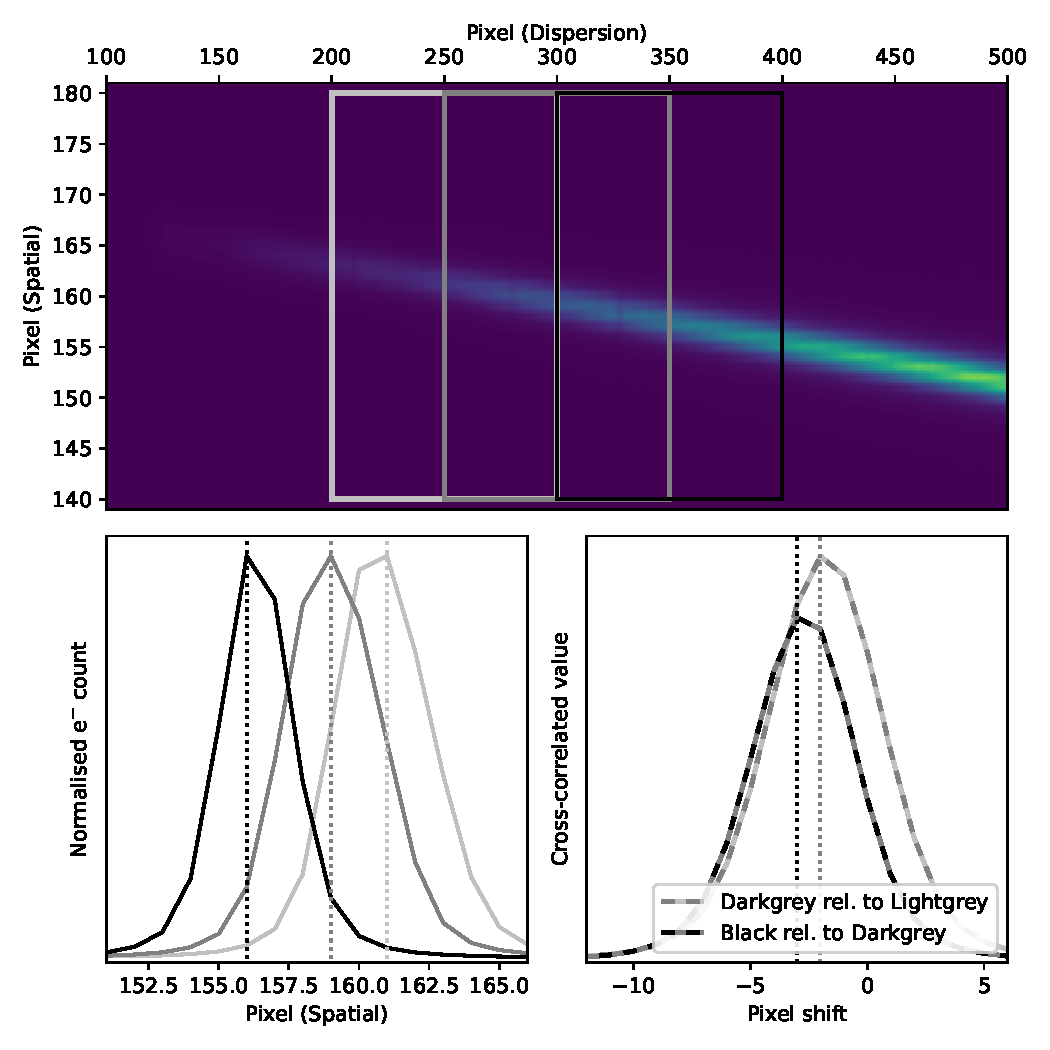
\includegraphics[width=\columnwidth]{fig_01_tracing.pdf}
    \caption{Top: A LT/SPRAT spectrum is rotated to illustrate how
    cross-correlation is used to find the shift between neighbouring
    sub-spectra. The orange, green and blue boxes are three examples
    sub-spectra. Bottom left: the three sub-spectra are summed in
    the dispersion direction to generate the three profiles that are
    cross-correlated to compute the shift. Bottom right: the
    cross-correlated function for the green sub-spectrum relative
    to the orange sub-spectrum (plotted in green), and the one
    for the blue sub-spectrum relative to the green sub-spectrum
    (plotted in blue).}
    \label{fig:trace}
\end{figure}


%%%%%%%%%%%%%%%%%%%%%%%%%%%%%%%%%%%%%%%%%%%%%%%%%%%%%%%%%%%%%%%%%%%%%%%%%%%%%%%%
\subsection{Image Rectification}
In some cases, a spectrum on the detector plane is not only tilted, but it is
also sufficiently distorted that the spatial and dispersion direction (in the
detector Cartesian coordinates) are no longer orthogonal to each other. While
this does not cause any complication in the tracing process, the extraction has
to be performed along a curve that the process is no longer a one dimensional
process. Without proper weighting in extracting flux at the sub-pixel level,
it can cause significant under- or over-subtraction of the sky background. More
complex methods have to be used to extract them directly
spectra~(e.g.\ \citet{2021A&A...646A..32P})), as implemented
in \textsc{PyReduce}. It can optimally extract such highly distorted spectra.
However, they cannot perform sky subtraction using the ``wings'' in the sky
region on either side of the line-spread profile. This has limited the usage
in a typical single-frame extraction without an accompanying sky observation
exposed using an identical slit setting. In \textsc{ASPIRED}, a
\texttt{TwoDSpec} object uses the spectral trace to align and resample the
spectral image in the spatial direction. By using the sky emission and the
coadded arc lines~(if available), it aligns and resamples the image in the
dispersion direction, so that the latter is performed on a spectrum~(nearly)
perfectly aligned with the detector x-y axes. Using the arc frame for this
process will deliver a more reliable rectification function.

%%%%%%%%%%%%%%%%%%%%%%%%%%%%%%%%%%%%%%%%%%%%%%%%%%%%%%%%%%%%%%%%%%%%%%%%%%%%%%%%
The rectification in the spatial direction \textbf{only} depends on the trace.
Each column of pixels gets (scaled and) shifted by resampling to align with the
centre of the spectrum. This usually leaves us with a spectrum tilted or curved
in the dispersion direction. Therefore, the same procedure for tracing the
spectra is applied in the spatial direction to find the best fit polynomial
solution for shifting (and scaling) in the dispersion direction for the second
step of the rectification process (See Fig.~\ref{fig:rectify}).

\begin{figure}
    \centering
    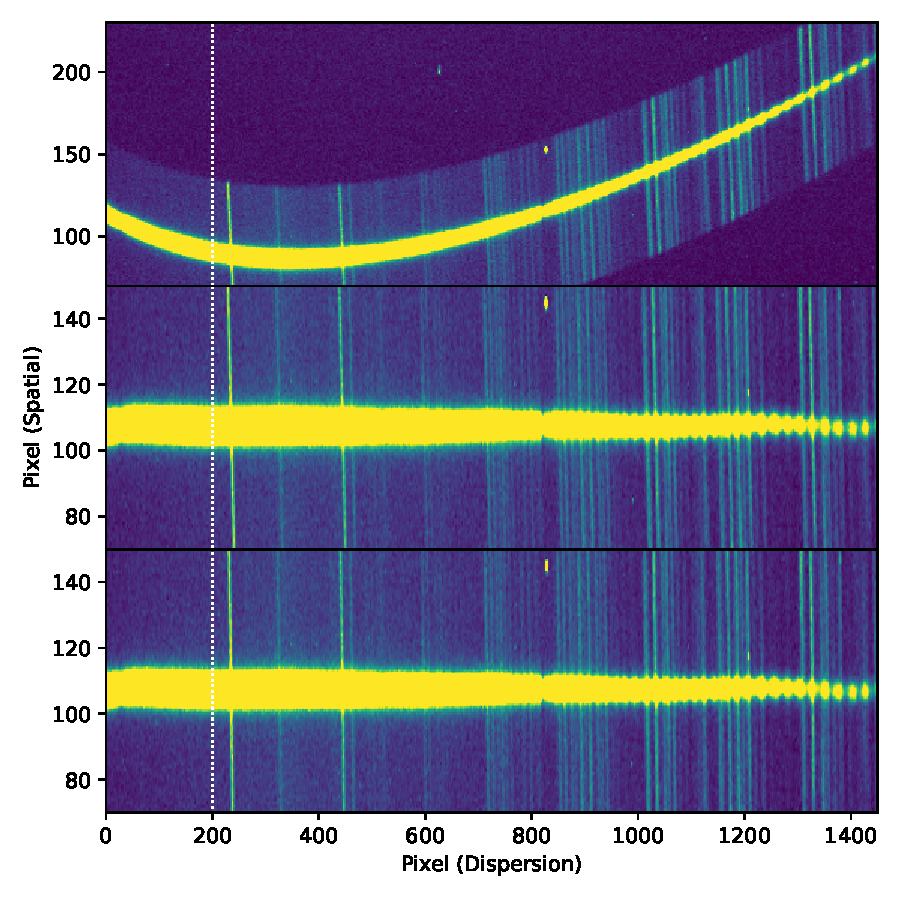
\includegraphics[width=\columnwidth]{fig_02_rectification.pdf}
    \caption{A two-dimensional spectrum from LCO/FLOYDS is used to demonstrate
    the rectification procedure. The dotted white line is aligned in the
    spatial direction to serve as a visual guide. Top: The trimmed image of a
    FLOYDS spectrum. Middle: The two-dimensional spectrum is resampled in the
    spatial direction based on the polynomial function of the trace. Bottom:
    The two-dimensional spectrum is resampled in the dispersion direction. The
    shifts and scales are found by cross-correlating the sub-spectra divided in
    the spatial direction. This is perpendicular to the tracing process.}
    \label{fig:rectify}
\end{figure}

%%%%%%%%%%%%%%%%%%%%%%%%%%%%%%%%%%%%%%%%%%%%%%%%%%%%%%%%%%%%%%%%%%%%%%%%%%%%%%%%
At the time of writing, this process is only possible if there is one trace. If
more than one trace is found/provided, only the first one will get processed.
The resampling is performed with \texttt{scipy.ndimage.zoom} which interpolates
with a cubic spline (the electron count is not perfectly conserved, but the
difference is small). It is possible to supply a set of pre-computed polynomials
to perform the rectification, which can significantly speed up the data
reduction process of a stable optical system. A change in the zeroth order
coefficient can shift the bluest part of the spectrum to the reddest part, and
vice versa. However, as long as the effect is identical in the science frame
and the standard frame they can be calibrated out or trimmed. Furthermore, the
edges of a detector are usually unusable, so it does not pose any real problem.

%%%%%%%%%%%%%%%%%%%%%%%%%%%%%%%%%%%%%%%%%%%%%%%%%%%%%%%%%%%%%%%%%%%%%%%%%%%%%%%%
\subsection{Spectral Extraction}
\label{sec:extract}
There are a few commonly used extraction methods; some work for
all kinds of spectral images, some only work with specific
observing strategies (e.g. the flat-relative optimal
extraction;~\citealt{2014A&A...561A..59Z}). The standard textbook
method is commonly called the \textit{top-hat} extraction or the
\textit{normal} extraction. It simply sums the electron counts over
a given size of the aperture, and is robust and easy to use. However,
this method does not deliver the maximal signal-to-noise ratio~(SNR)
from the available data. Various optimal extraction algorithms
can increase the SNR. This works by down-weighting the wings of the
spectral profile where almost all the photons are coming from the sky
rather than the source~(see Fig.~\ref{fig:extinction}). An optimal
extraction can boost the SNR, particularly for background-limited
sources, which are the case in most observations~(see
Fig.~\ref{fig:extraction_compared}). The extracted spectra and their
associated uncertainties and sky background counts can be plotted
for inspection. The residual image can also be exported for diagnostics.

\begin{figure}
    \centering
    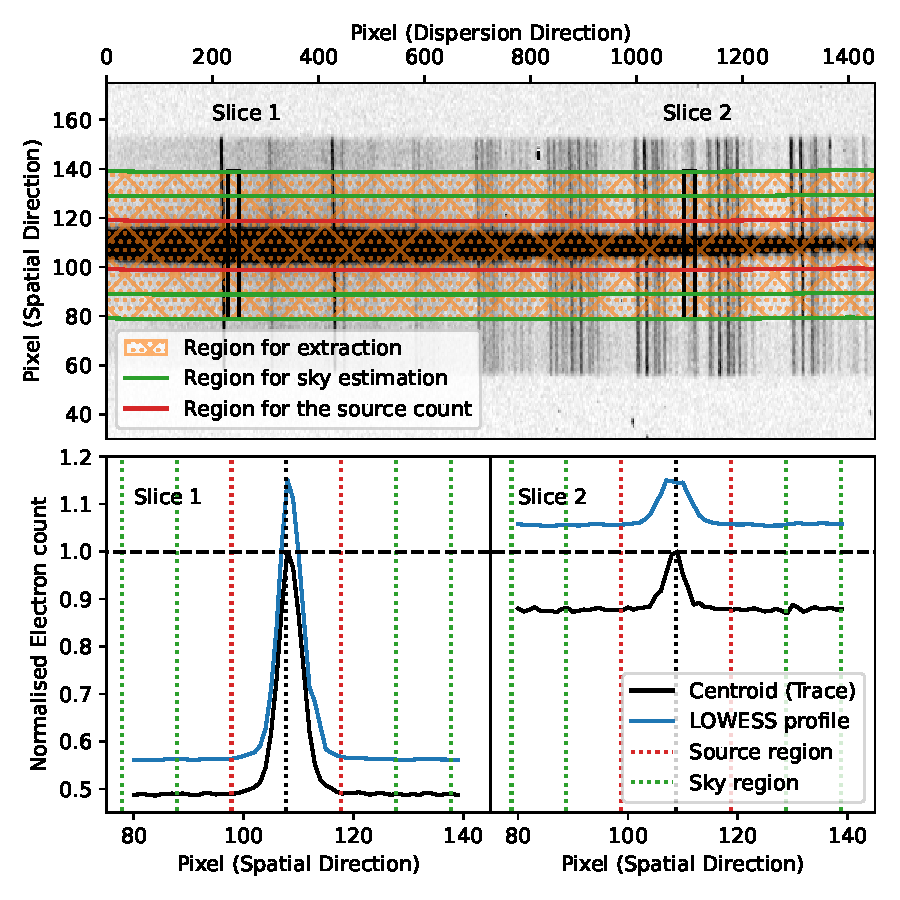
\includegraphics[width=\columnwidth]{fig_03_extraction_profile.pdf}
    \caption{The same spectrum as in Figure~\ref{fig:rectify} but the
    two-dimensional spectral image is slightly rotated to have the sky lines
    aligned with the spatial direction with the y-axis.
    Top: The regions used for source and sky extractions are marked
    by the red and green lines and arrows. The light shade of orange
    hash marks denotes the entire region that is used for spectral extraction.
    The two boxes show the two columns of pixels fitted with
    profiles in the bottom half of the figure (the boxes are inflated
    for clarity). Bottom: The electron counts across the two slices,
    The vertical black dashed line is the centroid~(trace) of the spectrum,
    the two red dashed lines mark the regions of the source and the
    pairs of green dashed lines on each side of the centroid are
    showing the regions used for sky extractions, respectively. The
    black line is the measured spectral profile (data), the blue
    line is the fitted LOWESS line-spread-function (model), offset for
    clarity.}
    \label{fig:extraction}
\end{figure}

%%%%%%%%%%%%%%%%%%%%%%%%%%%%%%%%%%%%%%%%%%%%%%%%%%%%%%%%%%%%%%%%%%%%%%%%%%%%%%%%
\subsubsection*{Tophat/Normal Extraction}
\label{sec:tophat}
The top-hat extraction does not weigh the pixels for extraction,
so every pixel has an equal contribution to the source count. Thus,
it is very robust in getting the total electron count across
a slice of pixels. The sky background count can be extracted
from the regions outside the extraction aperture to be
subtracted from the spectrum.

%%%%%%%%%%%%%%%%%%%%%%%%%%%%%%%%%%%%%%%%%%%%%%%%%%%%%%%%%%%%%%%%%%%%%%%%%%%%%%%%
\subsubsection*{Horne-86 Optimal Extraction}
\citet[hereafter H86]{1986PASP...98..609H} is the golden standard
of optimal extraction of spectra from modern electronic detectors.
We follow the H86 recipe except for the profile modelling,
where we provide three options: The first is a fixed Gaussian
profile, the second uses LOcally Weighted Scatterplot
Smoothing~\citep[LOWESS]{doi:10.1080/01621459.1979.10481038}
regression to fit for a polynomial, and the third accepts
a manually supplied profile.

%%%%%%%%%%%%%%%%%%%%%%%%%%%%%%%%%%%%%%%%%%%%%%%%%%%%%%%%%%%%%%%%%%%%%%%%%%%%%%%%
The default option is to use the Gaussian fit because it is
more robust against noise, cosmic ray contamination and detector
artefacts. It is particularly useful in extracting a faint
spectrum when the image is dominated by background noise as the
Gaussian profile is constructed from fitting the line-spread
function from the total stack of all the
sub-spectra~(as described in Sec.~\ref{sec:tracing}).
LOWESS, on the other hand, would do a better job in fitting
the profile of a resolved galaxy. In any case, the quality
of the extraction from a valid profile should be at least as
good as that performed with the top-hat extraction method.

%%%%%%%%%%%%%%%%%%%%%%%%%%%%%%%%%%%%%%%%%%%%%%%%%%%%%%%%%%%%%%%%%%%%%%%%%%%%%%%%
\subsubsection*{Marsh-89 Optimal Extraction}
\citet[hereafter M89]{1989PASP..101.1032M} improves on the H86 algorithm by
fitting the change in the shape and centroid of the profile from one end of the
spectrum to the other. It is very suited for extracting a highly tilted
spectrum where the tilting direction is aligned with \textbf{one} direction in
the $x$- or the $y$-axis of the detector. The algorithm still relies on the
assumption that the spatial and dispersion directions are orthogonal across
the entire frame (in the detector pixel coordinates). In \textsc{ASPIRED}, we
adapt Ian Crossfield's set of public \textsc{Python 2} code for
Astronomy\footnote{\url{https://people.ucsc.edu/~ianc/python/}}$^,$\footnote{\url{https://crossfield.ku.edu/python/}}
to \textsc{Python 3}.

\begin{figure}
    \centering
    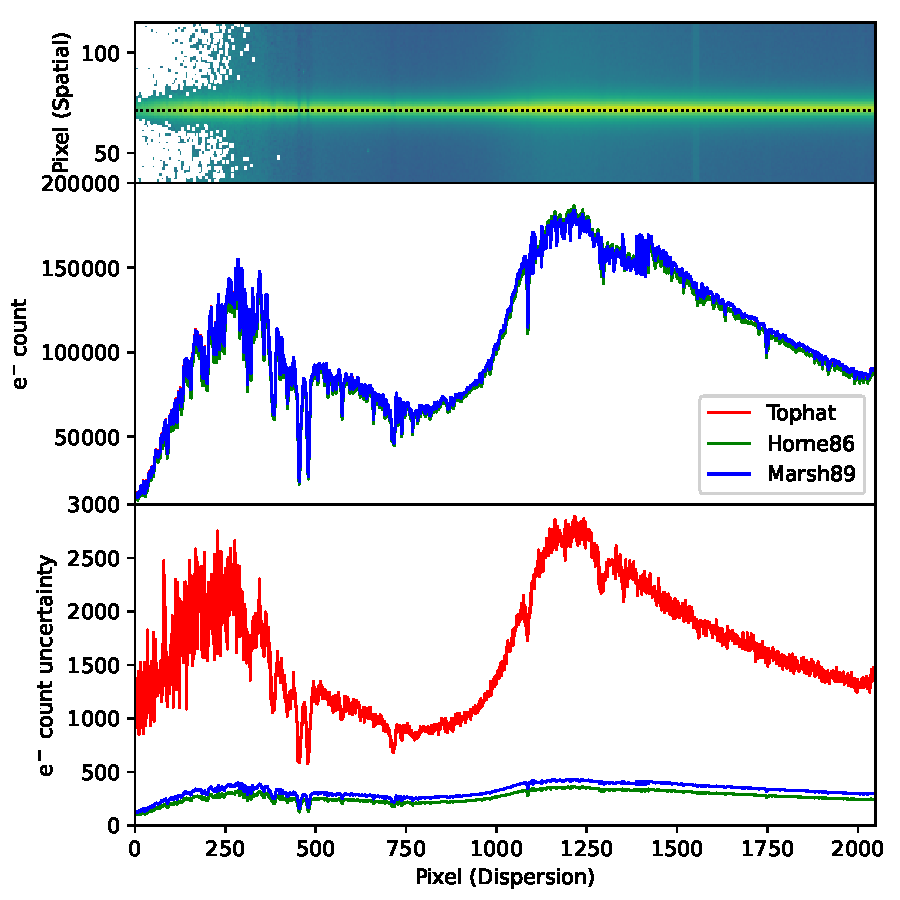
\includegraphics[width=\columnwidth]{fig_04_extraction_compared.pdf}
    \caption{Top: An LT/SPRAT spectrum of a featureless ultra-cool white dwarf PSO J1801+625~\citep{2020MNRAS.493.6001L}.
    Middle: The extracted spectra in electron counts using the three extraction methods
    are very similar. Bottom: The uncertainties with the three extraction methods
    in units of electron counts. The
    top-hat method is clearly noisier than the two optimal methods at the faint ends of the spectrum.}
    \label{fig:extraction_compared}
\end{figure}

%%%%%%%%%%%%%%%%%%%%%%%%%%%%%%%%%%%%%%%%%%%%%%%%%%%%%%%%%%%%%%%%%%%%%%%%%%%%%%%%
\subsection{Wavelength Calibration}
The wavelength calibration is powered by \textsc{RASCAL}, which is a concurrent
development to this work. All the public functions from \textsc{RASCAL} are
available in \textsc{ASPIRED} so users can have fine control over the
calibration. The diagnostic plots are the set provided by \textsc{RASCAL}.
They include the spectrum of the arc lamp where the traces on the science and
standard frames are, which also shows where the peaks are detected; the
peak-line pairs and the constrained space where the Hough-pairs are
selected~(see \citealt{2020ASPC..527..627V}); and a plot showing the fitting
solution, residual of the solution, and the pixel-wavelength relation~(
Fig.~\ref{fig:wavecal}).

The polynomial coefficients for the calibration can be supplied
directly, which would be useful for stable instruments in which
the variations in the dispersion are negligible. All the NIST lines
are available but we recommend providing arc lines manually.

\begin{figure}
    \centering
    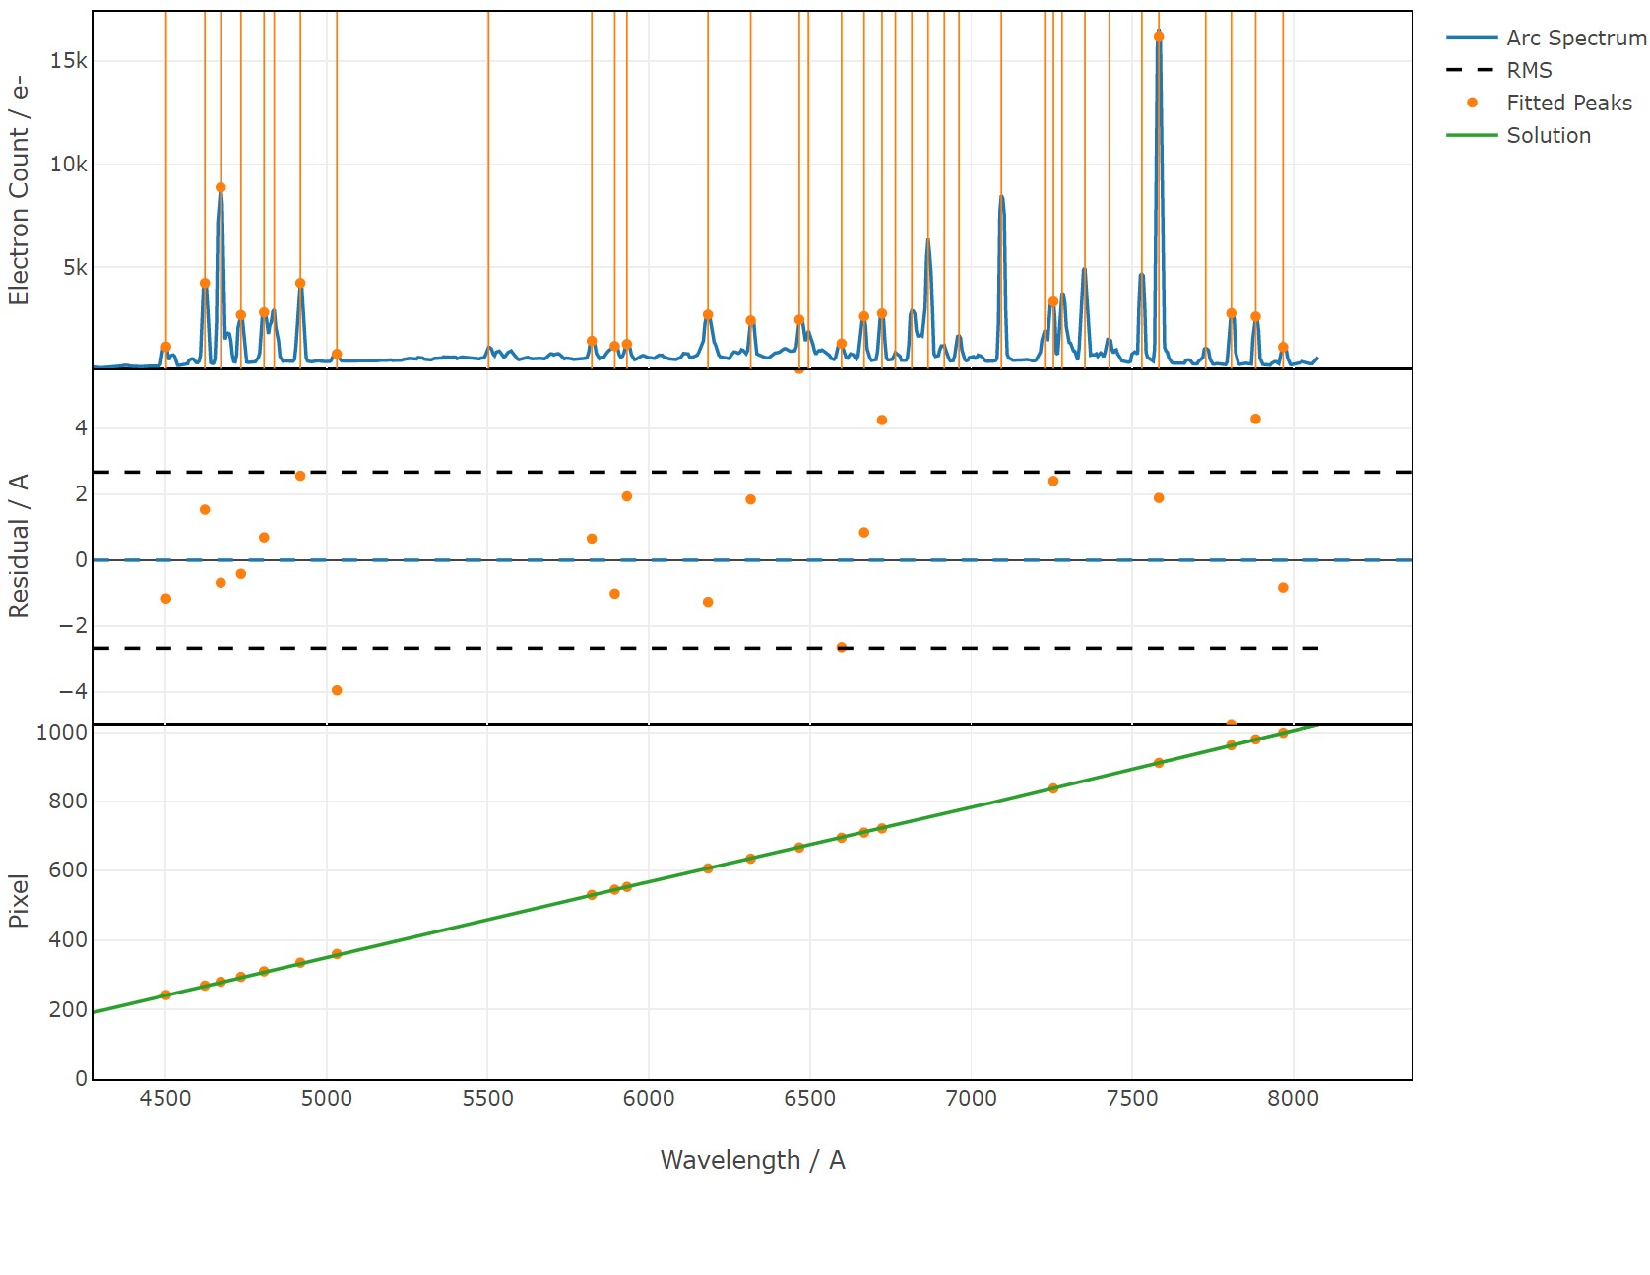
\includegraphics[width=\columnwidth]{fig_05_wavelength_calibration_diagnostics.pdf}
    \caption{The native wavelength calibration diagnostic plots from RASCAL.
    Top: the arc is plotted in blue, the fitted peaks are marked by
    the orange dots. Middle: The residual plot shows the difference
    between the fitted peaks and the true wavelengths. Bottom: The
    pixel-wavelength function (green) is overplotted with the fitted
    peaks (orange).}
    \label{fig:wavecal}
\end{figure}

%%%%%%%%%%%%%%%%%%%%%%%%%%%%%%%%%%%%%%%%%%%%%%%%%%%%%%%%%%%%%%%%%%%%%%%%%%%%%%%%
\subsection{Flux Calibration}
When a standard spectrum is wavelength calibrated, it can be
compared against literature values to obtain the sensitivity
function of the detector. All the standard stars available in
\textsc{iraf}\footnote{\url{https://github.com/iraf-community/iraf/tree/main/noao/lib/onedstds}}
and on the ESO webpage -- \textit{Optical and UV Spectrophotometric
Standard Stars}\footnote{\url{https://www.eso.org/sci/observing/tools/standards/spectra.html}}
are available on \textsc{ASPIRED}. We call the name of the set of data a
\textit{library}, and here is the complete listing of the source and reference
for each of the libraries where available:

\subsection*{European Southern Observatory~(ESO)}
The ESO standard spectra are grouped into five sets, they can be downloaded from \url{https://www.eso.org/sci/observing/tools/standards/spectra/}:

\begin{itemize}
    \item \texttt{esoctiostan} -- CTIO standards from \citet{1992PASP..104..533H, 1994PASP..106..566H}
    \item \texttt{esohststan} -- HST standards from \citet{1995AJ....110.1316B, 1996AJ....111.1743B}
    \item \texttt{esookestan} -- Oke standards from \citet{1990AJ.....99.1621O}
    \item \texttt{esowdstan} -- White dwarf standards from \citet{1995AJ....110.1316B}
    \item \texttt{esoxshooter} -- ESO X-shooter standards from \citet{2014Msngr.158...16M, 2014A&A...568A...9M}
\end{itemize}


\subsection*{Issac Newton Group of Telescopes~(ING)}

The ING listing is grouped into five sets by the last name of the authors\footnote{\url{http://www.ing.iac.es/Astronomy/observing/manuals/html_manuals/tech_notes/tn065-100/workflux.html}}.

\begin{itemize}
    \item \texttt{ing\_oke} -- \citet{1990AJ.....99.1621O} standards
    \item \texttt{ing\_sto} -- \citet{1977ApJ...218..767S} standards
    \item \texttt{ing\_og} -- \citet{1965ApJ...141...83E} standards
    \item \texttt{ing\_mas} -- \citet{1988ApJ...328..315M} standards
    \item \texttt{ing\_fg} -- \citet{1984PASP...96..530F} standards
\end{itemize}

\subsection*{\texttt{iraf} Standards}
The complete listing of \texttt{iraf} standards can be found at
\url{https://github.com/iraf-community/iraf/tree/main/noao/lib/onedstds}.
References are included is they are available.

\begin{itemize}
    \item \texttt{irafblackbody}
    \item \texttt{irafbstdscal} -- KPNO IRS standards (i.e.\ those from the Henry Draper~(HD) catalogue)
    \item \texttt{irafctiocal} -- The original CTIO standards \citet{1983MNRAS.204..347S, 1984MNRAS.206..241B}
    \item \texttt{irafctionewcal} -- The updated CTIO standards \citet{1992PASP..104..533H, 1994PASP..106..566H}
    \item \texttt{irafiidscal} -- KPNO IIDS standards \citet{1988ApJ...328..315M}
    \item \texttt{irafirscal} -- KPNO IRS standards \citet{1988ApJ...328..315M}
    \item \texttt{irafoke1990} -- HST standards \citet{1990AJ.....99.1621O}
    \item \texttt{irafredcal} -- KPNO IRS standards \& IIDS \citet{1988ApJ...328..315M} with wavelength beyond 8\,370\,$\mathrm{\AA}$
    \item \texttt{irafspechayescal} -- KPNO standards \citet{1988ApJ...328..315M}
    \item \texttt{irafspec16cal} -- CTIO standards \citet{1992PASP..104..533H, 1994PASP..106..566H} at 16$\mathrm{\AA}$ interval
    \item \texttt{irafspec50cal} -- KPNO standards \citet{1988ApJ...328..315M, 1990ApJ...358..344M} at 50$\mathrm{\AA}$ interval
\end{itemize}



The calibration can be done in either AB magnitude or
flux density~(per unit wavelength). The two should give similar
results, but the response functions found would not be equivalent
because fitting to magnitudes is in logarithmic space and smoothing~(see
below) will have a different effect compared to flux fitting.

%%%%%%%%%%%%%%%%%%%%%%%%%%%%%%%%%%%%%%%%%%%%%%%%%%%%%%%%%%%%%%%%%%%%%%%%%%%%%%%%
\subsubsection*{Smoothing}
A Savitzky-Golay smoothing
filter\footnote{\url{https://docs.scipy.org/doc/scipy/reference/generated/scipy.signal.savgol_filter.html}}~\citep[hereafter, SG-filter]{1964AnaCh..36.1627S}
can be applied to the data before computing the sensitivity curve. This function
works by fitting low-order polynomials to localised subsets of the data to
suppress noise in the data at each point interval. It is similar to the
commonly used median boxcar filter, but uses more weighted information to
retain information better while removing noise. This can be used independently
or with continuum fitting (see below), which uses a LOWESS filter. By default,
the SG-filter removes only significant noise~(e.g.\ those from unsubtracted
cosmic rays).

%%%%%%%%%%%%%%%%%%%%%%%%%%%%%%%%%%%%%%%%%%%%%%%%%%%%%%%%%%%%%%%%%%%%%%%%%%%%%%%%
\subsubsection*{Continuum Fitting}
By default, the continuum of the standard spectrum is found for deriving the
sensitivity curve. However, this process is strongly dependent on both the
resolution of the literature and the observed standards, as well as the
absorption lines in 

%%%%%%%%%%%%%%%%%%%%%%%%%%%%%%%%%%%%%%%%%%%%%%%%%%%%%%%%%%%%%%%%%%%%%%%%%%%%%%%%
This process is used after the smoothing procedure~(if performed). The continuum
is found by fitting the standard spectrum with a LOWESS function as described in
Sec.~\ref{sec:extract}. This can remove any outlying random noise and absorption
lines when computing the sensitivity. Users are reminded to be cautious with
this procedure as removing the absorption features in computing the sensitivity
function can significantly affect the flux calibration near the absorption
features.

%%%%%%%%%%%%%%%%%%%%%%%%%%%%%%%%%%%%%%%%%%%%%%%%%%%%%%%%%%%%%%%%%%%%%%%%%%%%%%%%
\subsubsection*{Sensitivity Function}
The sensitivity curve is computed by dividing the observed standard spectrum by
the literature one and then interpolating the result using a spline or a
polynomial function~(Fig.~\ref{fig:fluxcal}. This can be done with or without
any pre-smoothing and/or continuum fitting. In case of a high-resolution
literature standard spectrum~(e.g.\ the ESO X-Shooter standards), the
absorption line profiles should be used as part of the sensitivity computation.
While in the case of the standard stars from \citep{1990AJ.....99.1621O},
they have removed absorption lines when producing the standard spectra, a
smooth continuum of the observed spectrum should be used for computing
the sensitivity function. Users can also manually supply a sensitivity function
as a callable function that accepts a wavelength value and returns the $\log$
of the sensitivity value at that wavelength. When such a curve is provided
manually, it is assumed to be in the unit of flux per second.

\begin{figure}
    \centering
    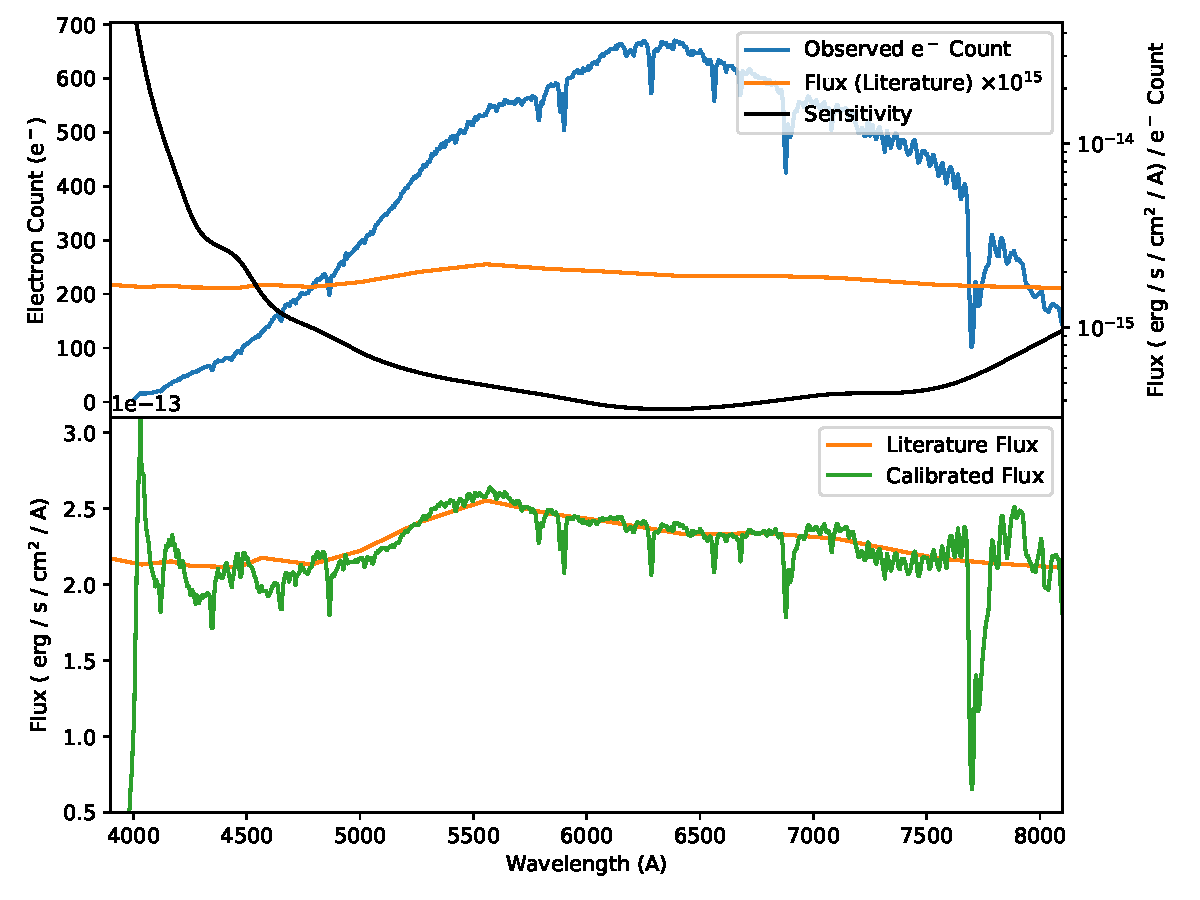
\includegraphics[width=\columnwidth]{fig_06_flux_calibration_diagnostics.pdf}
    \caption{Top: The extracted standard spectrum in electron counts
    (blue), the literature spectrum in units of flux density (multiplied
    by $10^{17}$; colour), and the sensitivity function (y-axis on the right; black).
    Bottom: The literature spectrum (same as the one above) is plotted
    in orange, and the calibrated observed spectrum is plotted in green.}
    \label{fig:fluxcal}
\end{figure}

%%%%%%%%%%%%%%%%%%%%%%%%%%%%%%%%%%%%%%%%%%%%%%%%%%%%%%%%%%%%%%%%%%%%%%%%%%%%%%%%
\subsection{Atmospheric Extinction Correction}
\textsc{ASPIRED} currently has four built-in atmospheric extinction curves:

\begin{enumerate}
    \item Roque de los Muchachos Observatory~(2\,420\,m)\footnote{\url{http://www.ing.iac.es/astronomy/observing/manuals/ps/tech\_notes/tn031.pdf}}
    \item Mauna Kea Observatories~\citep[4\,205\,m;][]{2013A&A...549A...8B}
    \item Cerro Paranal Observatory~\citep[2\,635\,m;][]{2011A&A...527A..91P}
    \item La Silla Observatory~(2\,400\,m)\footnote{\url{https://www.eso.org/public/archives/techdocs/pdf/report\_0003.pdf}}
\end{enumerate}

It reports the extinction in magnitude per airmass as a function of wavelength,
roughly between $3\,000$ and $10\,000$\,\AA. Alternatively, a callable function
in the appropriate units can be supplied to perform the extinction correction.
The airmass of the observation can be found from the header if it is reported
using the conventional keywords for airmass. See Figure~\ref{fig:extinction}
for a comparison plot of the atmospheric extinction curves.

\begin{figure}
    \centering
    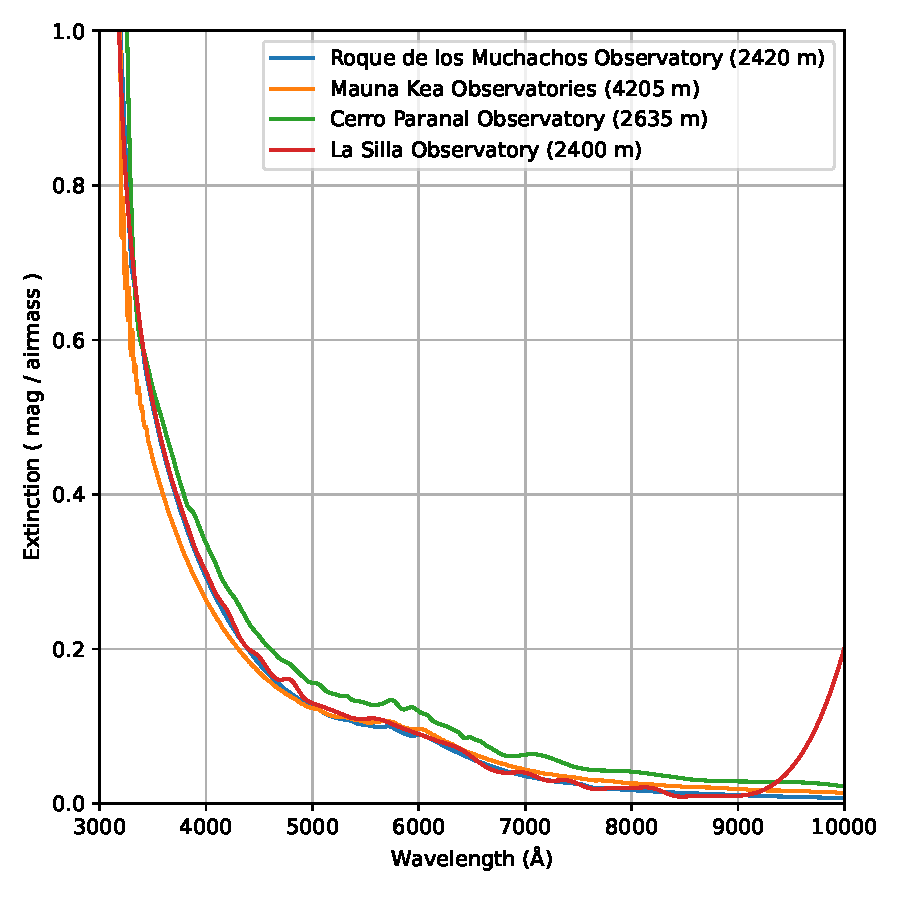
\includegraphics[width=\columnwidth]{fig_07_extinction_curves.pdf}
    \caption{The extinction curves measured at the four sites: Roque de los
    Muchachos Observatory~(2420\,m; blue), Mauna Kea Observatories~(4\,205\,m;
    orange), Cerro Paranal Observatory~(2\,635\,m; green), and La Silla
    Observatory~(2400\,m; red). The extinction table of La Silla Observatory
    terminates at $9\,000$\,\AA. The rise at the red end of the curve is an
    undesired artefact due to extrapolation using a cubic spline. We are
    explicitly plotting this range to serve as a warning since we opt to
    preserve the raw data as provided without appending fake data points.}
    \label{fig:extinction}
\end{figure}

%%%%%%%%%%%%%%%%%%%%%%%%%%%%%%%%%%%%%%%%%%%%%%%%%%%%%%%%%%%%%%%%%%%%%%%%%%%%%%%%
\subsection{Telluric Absorption Removal}
During the process of generating the sensitivity function, masks are used
over the Telluric regions to generate the Telluric absorption
profile from the standard star. The default masking regions are $6\,850-6\,960$
and $7\,580-7\,700$\ \AA\ only. This profile can then be multiplied
by a factor to be determined in order to remove the Telluric absorption
features in the science target. The best multiplicative factor is found
by minimising the difference between the continuum and the Telluric-absorption
corrected spectrum simultaneously for all the Telluric absorption features.
An \textbf{extra} multiplier can be manually provided to adjust the
strength of the subtraction. This is designed for manually fine-tuning the
absorption factor; otherwise, it defaults to $1.0$.

%%%%%%%%%%%%%%%%%%%%%%%%%%%%%%%%%%%%%%%%%%%%%%%%%%%%%%%%%%%%%%%%%%%%%%%%%%%%%%%%
\subsection{Resample}
All the operations above are performed as a function of the native detector
pixels. Including the telluric absorption corrections as the telluric profile
is generated in the standard spectrum pixel/wavelength coordinates, the
correction applied to the target spectrum is performed using an interpolated
function of the profile at the wavelengths of the target spectrum. Many legacy
software can only read the spetrum using the header information to create
the wavelength cooridnates using only three parameter: the wavelength of the
first element of the spectral array, the bin width of each wavelength
coordinate, and the length of the spectral array. This requires a uniformly
sampled wavelength axis, which never happens naturally as there is always some
level of of image distortion at the detector plane. A resampling is necessary
to turn the data into such format.

The resampling is performed with the \textsc{spectres} package. Although
this package allows non-uniform wavelength spacing resampling, we are only
using it for uniform resampling for the purpose of exporting the data as FITS
files.

%%%%%%%%%%%%%%%%%%%%%%%%%%%%%%%%%%%%%%%%%%%%%%%%%%%%%%%%%%%%%%%%%%%%%%%%%%%%%%%%
\subsection{Export}
At the time of writing, 22 types of output to CSV and FITS files are supported.
Each CSV will have the data stored in a separate column, while the FITS has
the data stored in a separate Header Data Unit~(HDU). Each spectrum is exported
as a separate file. The options are:

\begin{enumerate}
    \item \texttt{trace} -- two columns/HDUs containing the pixel coordinates
    of the trace and its width.
    \item \texttt{count} -- three columns/HDUs containing the electron count
    of the spectrum, its uncertainty, and the sky background.
    \item \texttt{weight\_map} -- one column/HDU for the extraction profile,
    in top hat and \texttt{horne86} extraction this is a one dimensional array,
    while the \texttt{marsh90} extraction returns a two dimensional array.
    \item \texttt{arc\_spec} -- three columns/HDUs for one dimensional arc
    spectrum, pixel coordinates of the arc line position (sub-pixel precision),
    and the pixel coordinates of the arc line effective position~(
    e.g.\ accounted for chip gaps).
    \item \texttt{wavecal} -- one column/HDU for the Polynomial coefficients
    for wavelength calibration. The header contains the information of the
    polynomial type.
    \item \texttt{wavelength} -- one column/HDU for the wavelength at the
    native pixel position as extracted.
    \item \texttt{sensitivity} -- one column/HDU containing the sensitivity
    function of the detector as a function of the native detector pixel
    \item \texttt{flux} -- three columns/HDUs containing the
    flux of the spectrum, its uncertainty, and the sky background.
    \item \texttt{atm\_ext} -- one column/HDU containing the atmospheric
    extinction correction factor at each wavelength position.
    \item \texttt{flux\_atm\_ext\_corrected} -- three columns/HDUs containing
    the atmospheric extinction corrected flux of the spectrum, its
    uncertainty, and the sky background,
    \item \texttt{telluric\_profile} -- one column/HDU containing the telluric
    absorption profile from the standard spectrum.
    \item \texttt{flux\_telluric\_corrected} -- three columns/HDUs containing
    the telluric absorption corrected flux, uncertainty, and the sky
    background.
    \item \texttt{flux\_atm\_ext\_telluric\_corrected} -- three columns/HDUs
    containing the atmospheric extinction and telluric corrected flux,
    uncertainty, and the sky background.
    \item \texttt{wavelength\_resampled} -- one column/HDU containing the
    wavelength at each resampled position.
    \item \texttt{count\_resampled} -- three columns/HDUs containing the
    electron count of the spectrum, its uncertainty, and the sky background
    being subtracted during the extraction process at the resampled wavelength.
    \item \texttt{sensitivity\_resampled} -- one column/HDU containing the
    sensitivity function of the detector as a function of resampled wavelength.
    \item \texttt{flux\_resampled} -- three columns/HDUs containing the
    flux of the spectrum, its uncertainty, and the sky background at the
    resampled wavelength.
    \item \texttt{atm\_ext\_resampled} -- one column/HDU containing the
    atmospheric extinction correction factor at the resampled wavelength.
    \item \texttt{flux\_resampled\_atm\_ext\_corrected} -- three columns/HDUs
    containing the atmospheric extinction corrected flux of the spectrum, its
    uncertainty, and the sky background at the resampled wavelength.
    \item \texttt{telluric\_profile\_resampled} -- one column/HDU containing
    the telluric absorption profile from the standard spectrum at the resampled
    wavelength.
    \item \texttt{flux\_resampled\_telluric\_corrected} -- three columns/HDUs
    containing the telluric absorption corrected flux, uncertainty, and the sky
    background at the resampled wavelength.
    \item \texttt{flux\_resampled\_atm\_ext\_telluric\_corrected} -- three
    columns/HDUs containing the atmospheric extinction and telluric absorption
    corrected flux, uncertainty, and the sky background at the resampled
    wavelength.
\end{enumerate}


%%%%%%%%%%%%%%%%%%%%%%%%%%%%%%%%%%%%%%%%%%%%%%%%%%%%%%%%%%%%%%%%%%%%%%%%%%%%%%%%
\section{Example Data Reduction Product}
\label{sec:examples}
Being a flexible toolkit, \texttt{ASPIRED} is not designed to reduce data for a
specific instrument. Instead, it can be customised to suit many configurations,
as long as they are long-slit-like. We demonstrate that with data products
from nine different instruments, most of them have conventional long-slit settings.
In the case of Gemini/GMOS, it has a single spectrum exposed onto three detectors,
each is read out with 4 amplifiers. The bias subtraction is also unconventional,
so all the image data reduction procedures have to be done outside of ASPIRED
beforehand. We compare the reduction against the official one for the kilonova
event AT 2017gfo\footnote{\url{https://www.wiserep.org/}}~\citep{2017ApJ...848L..32M}. Las Cumbres
Observatory/FLOYDS has a beam-splitter to expose
the first order red beam and the second order blue beam into two non-parallel
curved spectra on a single chip. Both the northern and southern FLOYDS suffers
from strong fringing effects. This is not handled by ASPIRED natively as well,
so the correction was done by directly accessing the intermediate data stored
inside the \texttt{OneDSpec} object. iPTF14hls, an SN II-P with strong emission
lines is used as an example for comparison~\citep{2017Natur.551..210A}. The Liverpool Telescope/SPRAT is a
high throughput low-resolution spectrograph with a conventional optical design;
in this case, we compare the reduction of a nova shell DO Aql from a stack of
four individual exposures\footnote{\url{https://telescope.livjm.ac.uk/cgi-bin/lt_search}}~\citep{2020MNRAS.499.2959H}. The Very Large Telescope/FORS2 data of a helium
accretor~(AM CVn) V418 Ser stacked from 21 individual exposures is used as our
last comparison~\citep{2020MNRAS.496.1243G}. The first three were compared against data reduction from
\textsc{iraf}-based pipelines, while the last one is reduced with Molly\footnote{\url{https://cygnus.astro.warwick.ac.uk/phsaap/software/molly/html/INDEX.html}}~\citep{2019ascl.soft07012M}, which
is built on top of STARLINKs. All of the spectra are resampled to match the
published spectra.

%%%%%%%%%%%%%%%%%%%%%%%%%%%%%%%%%%%%%%%%%%%%%%%%%%%%%%%%%%%%%%%%%%%%%%%%%%%%%%%%
WHT/ISIS and ACAM demonstrate an extremely low signal-to-noise reduction of an ultra-cool
white dwarf with a smooth blackbody-like spectrum~\citep{2020MNRAS.493.6001L}.
The tracing and extraction are only possible after careful cosmic ray removal
and trimming of the images. The spectral shape of the ISIS spectra in both the
blue and red arm are in good agreement with the ACAM spectrum. The TNG/DOLORES
shows a simultaneous tracing of two targets separated by 5" incidented on the
long-slit in a single exposure, followed by sequential extraction. The
GTC/OSIRIS works on a blue large amplitude pulsator with many resolved
absorption lines in both the science and the standard targets~(Feige
110\footnote{\url{https://www.eso.org/sci/observing/tools/standards/spectra/feige110.html}}; ~\citealp{2022MNRAS.511.4971M}). 

%%%%%%%%%%%%%%%%%%%%%%%%%%%%%%%%%%%%%%%%%%%%%%%%%%%%%%%%%%%%%%%%%%%%%%%%%%%%%%%%
\begin{table*}
    \centering
    \begin{tabular}{l|c|c|c}\hline
        Telescope/Instrument & Object Type                                 & Grating             & Arc \\\hline\hline
        \multicolumn{4}{c}{Conventional Long-slit Setup}\\\hline
        Liverpool/SPRAT      & Nova shell remnant (DO Aql)                 & 600\,l/mm           & Xe \\
        GTC/OSIRIS           & BLAP (ZGP-BLAP-09)                          & R2500U \& R1000B    & HgArNe \\
        VLT/FORS             & AM CVn (V418 Ser)                           & 600B                & HeHgCd \\
        TNG/DOLORES          & Common Proper Motion System (dM + dMWD)     & LR-B                & ArKrNeHg \\
        WHT/ISIS             & Ultracool White Dwarf (PSO J1801+625)       & R300B \& R300R      & CuAr \\
        WHT/ACAM             & Ultracool White Dwarf (PSO J1801+625)       & V400                & CuAr \\\hline
        \multicolumn{4}{c}{Other Setup}\\\hline
        Gemini/GMOS          & kilonova (AT 2017gfo)                       & R400 \& B600        & CuAr \\
        LCO/FLOYDS           & Type II-P (iPTF14hls)                       & 235\,l/mm           & HgArZn \\\hline
\end{tabular}
    \caption{List of the eight targets used in Fig.~\ref{fig:extraction_compared} \& \ref{fig:use_cases}. See body text for refereces.}
    \label{tab:my_label}
\end{table*}

%%%%%%%%%%%%%%%%%%%%%%%%%%%%%%%%%%%%%%%%%%%%%%%%%%%%%%%%%%%%%%%%%%%%%%%%%%%%%%%%
\begin{figure*}
    \centering
    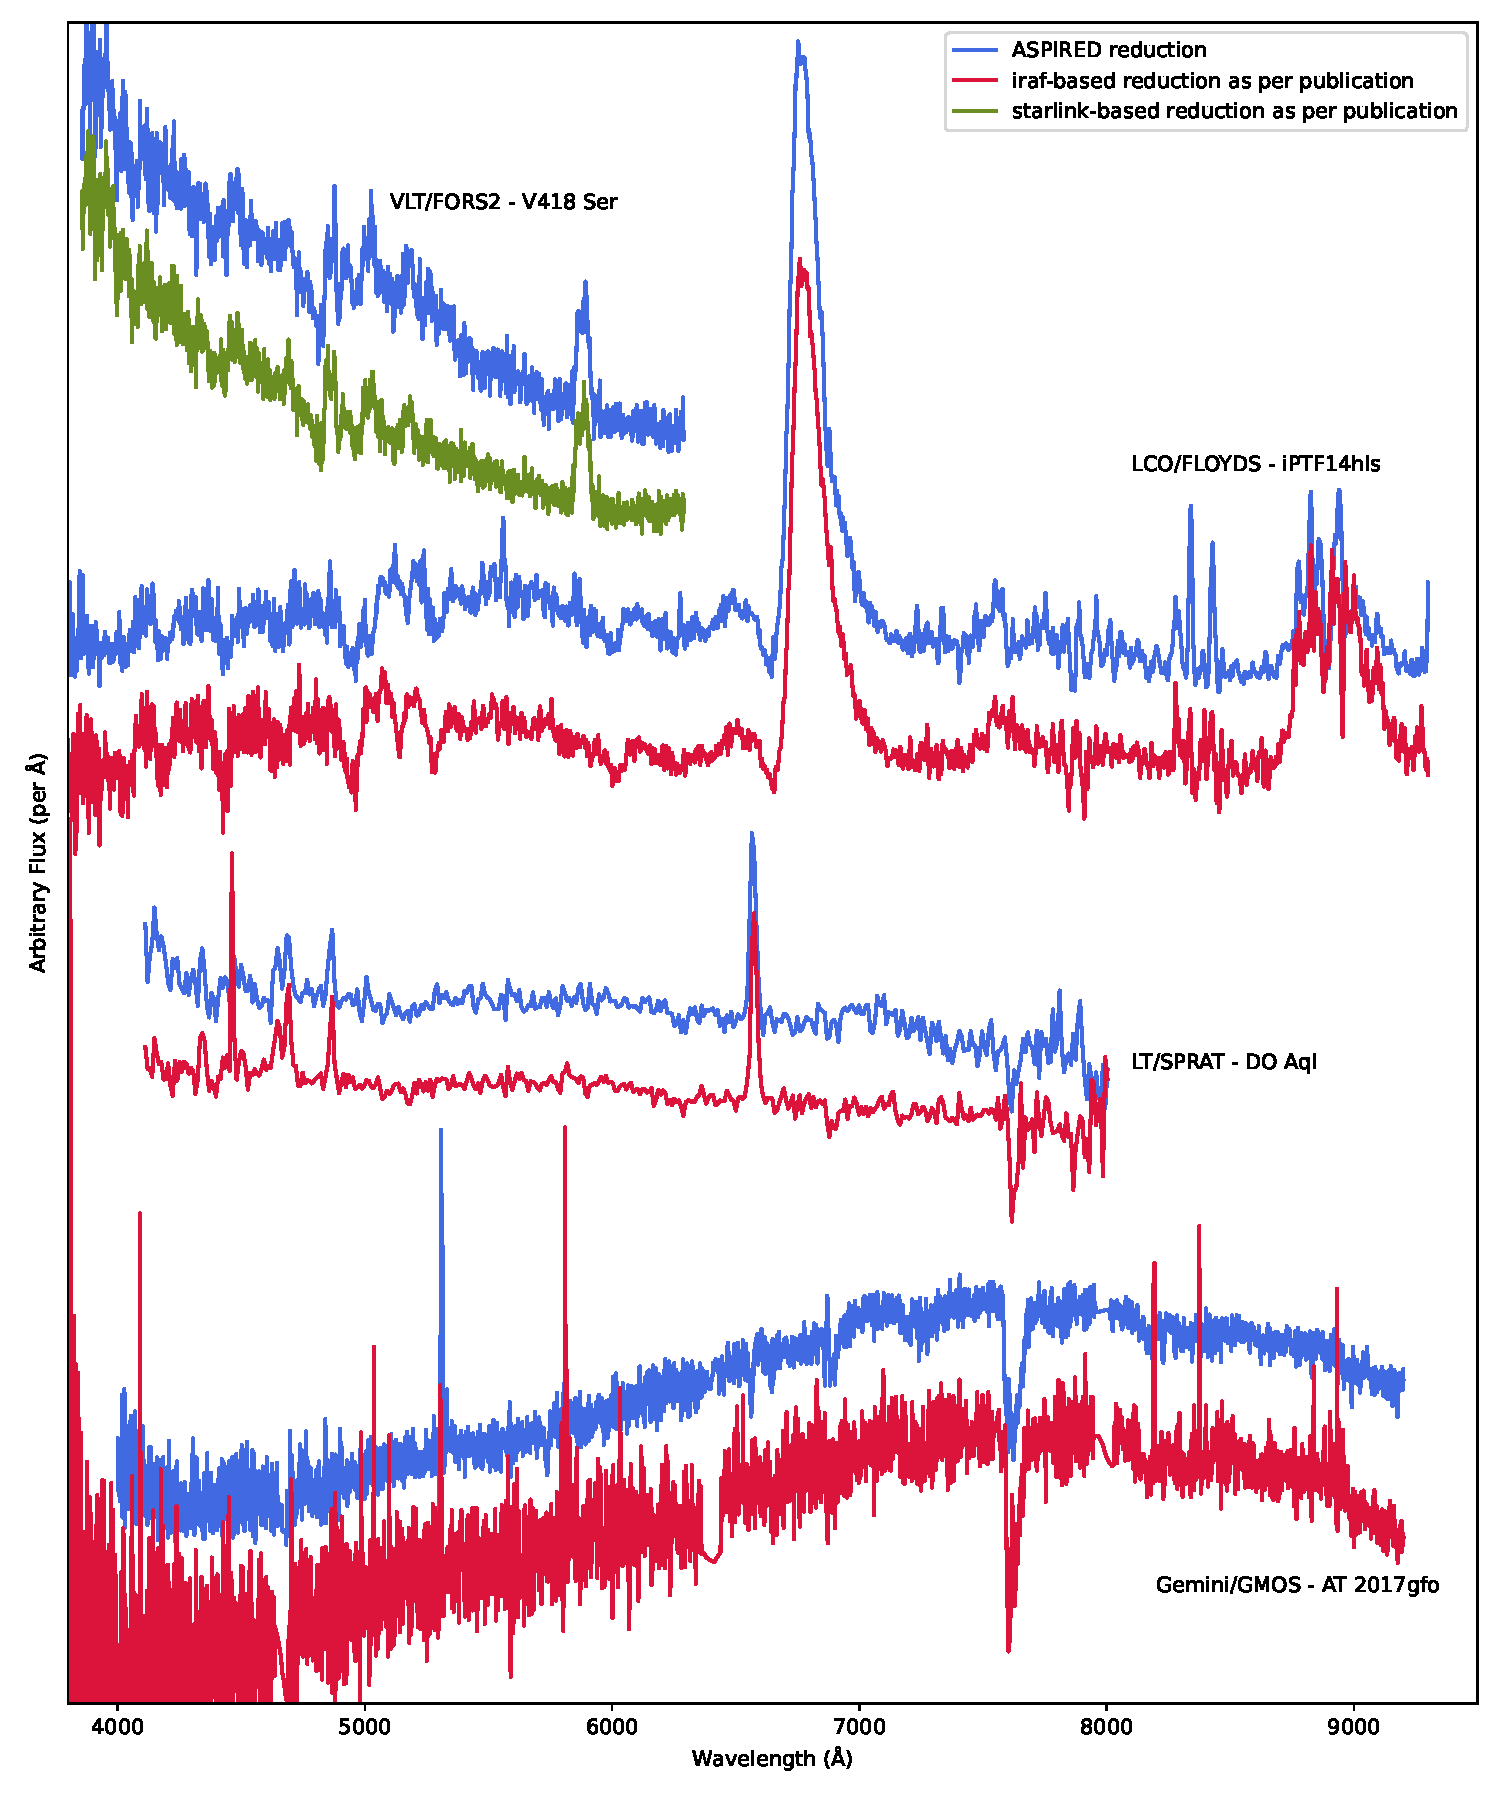
\includegraphics[width=\textwidth]{fig_08_reduction_compared.pdf}
    \caption{From top to bottom are the comparison spectra taken with VLT/FORS2,
    LCO/FLOYDS, LT/SPRAT and Gemini/GMOS in long-slit mode. The published FORS2
    spectrum was reduced using \textsc{Molly}~(green) powered by the \textsc{STARLINK}
    library. The other three (red) were reduced using the respective \textsc{iraf}-based
    pipelines. All spectra reduced with \textsc{ASPIRED}~(blue) are resampled to match
    the respective published spectra. Telluric correction is applied using the default
    setting.}
    \label{fig:reduction_compared}
\end{figure*}

\begin{figure*}
    \centering
    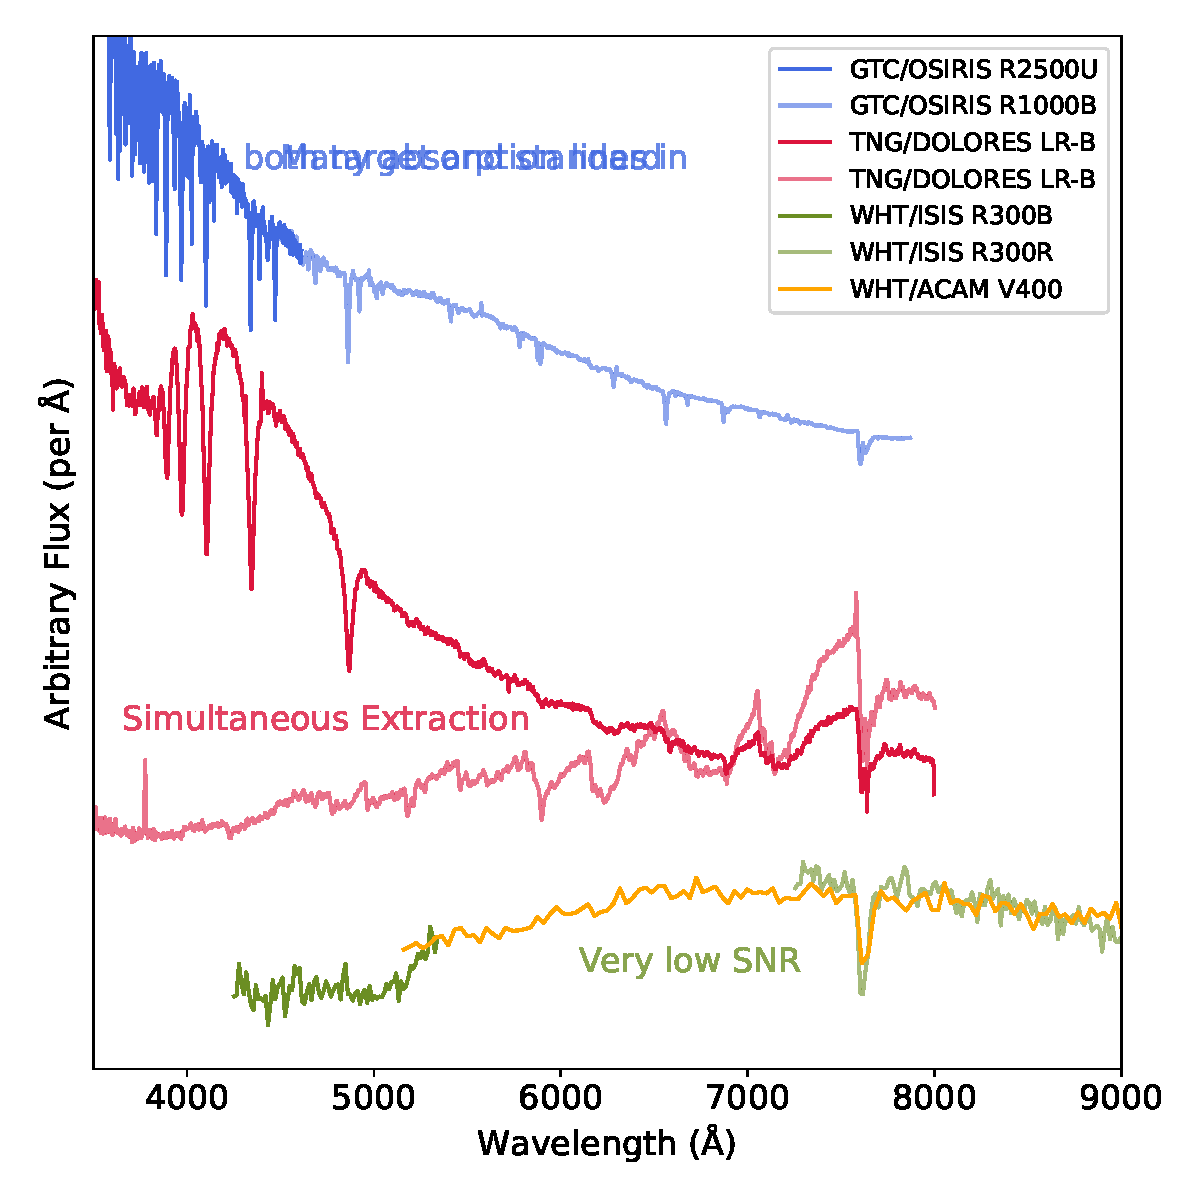
\includegraphics[width=\textwidth]{fig_09_use_case_plots.pdf}
    \caption{Example extractions of some special cases. The GTC/OSIRIS (blue hue)
    spectra were flux calibrated in the shorter wavelengths where there are a lot
    of absorption features. The TNG/DOLORES spectra were of two targets where the
    tracing was done simultaneously and then the extraction done~(red hue)
    sequentially. The WHT/ISIS and ACAM (green hue and yellow) are extracting a
    target with very low signal-to-noise ratio.}
    \label{fig:use_cases}
\end{figure*}

%%%%%%%%%%%%%%%%%%%%%%%%%%%%%%%%%%%%%%%%%%%%%%%%%%%%%%%%%%%%%%%%%%%%%%%%%%%%%%%%
\section{Distribution}
\label{sec:distribution}

\textsc{ASPIRED} is released under the BSD (3-Clause) License. The
source code is hosted on \textsc{Github}, which can be found at
\url{https://github.com/cylammarco/ASPIRED}. The DOI of each version
can be found at \textsc{zenodo}: \url{https://zenodo.org/record/4463569#.YLjdrKgzYrQ}.
For more straightforward installation, \textsc{ASPIRED} is also available at Python
Package Index~(PyPI): \url{https://pypi.org/project/aspired} so
users can install the software by a simple command of 
\begin{verbatim}
>> pip install aspired.
\end{verbatim}
While the latest stable version can be installed with
\begin{verbatim}
>> pip install git+https://github.com/
    cylammarco/ASPIRED@main
\end{verbatim},
and the latest development version can be installed with 
\begin{verbatim}
>> pip install git+https://github.com/
    cylammarco/ASPIRED@dev-v[X].[Y].X
\end{verbatim}. Where \verb+[X]+ and \verb+[Y]+ are the major and minor version numbers,
\verb+X+ is an actual character of the branch name to denote it as a patch-level maintenance
branch.

It is also possible to clone the entire repository
and install with the setup script with
\begin{verbatim}
>> git clone [url to main/dev/a specific commit]
>> python setup.py
\end{verbatim}
.

%%%%%%%%%%%%%%%%%%%%%%%%%%%%%%%%%%%%%%%%%%%%%%%%%%%%%%%%%%%%%%%%%%%%%%%%%%%%%%%%
\section{Summary and Future work}
\label{sec:summary}

%%%%%%%%%%%%%%%%%%%%%%%%%%%%%%%%%%%%%%%%%%%%%%%%%%%%%%%%%%%%%%%%%%%%%%%%%%%%%%%%
\section*{Acknowledgements}
This work was partially supported by OPTICON. This project has
received funding from the European Union's Horizon 2020 research and
innovation programme under grant agreement No 730890. This material
reflects only the authors' views and the Commission is not liable for
any use that may be made of the information contained therein.

This work was partially supported by the Polish NCN grant Daina
No. 2017/27/L/ST9/03221.

MCL is supported by a European Research Council (ERC) grant under the European Union's Horizon 2020 research and innovation program (grant agreement number 852097).

IA is a CIFAR Azrieli Global Scholar in the Gravity and the Extreme Universe Program and acknowledges support from that program, from the ERC under the European Union's Horizon 2020 research and innovation program (grant agreement number 852097), from the Israel Science Foundation (grant number 2752/19), from the United States - Israel Binational Science Foundation (BSF), and from the Israeli Council for Higher Education Alon Fellowship.

The LT is operated on the island of La Palma by Liverpool
John Moores University in the Spanish Observatorio del Roque
de los Muchachos of the Instituto de Astrof{\'i}sica de Canarias with
financial support from the UK Science and Technology Facilities
Council.

This work makes use of observations from the Las Cumbres Observatory
global telescope network. We have made use of the data collected from
the FLOYDS spectrograph on the LCOGT 2m telescope at both Siding Spring,
Australia and Maui, HI, United States.
%%%%%%%%%%%%%%%%% APPENDICES %%%%%%%%%%%%%%%%%%%%%

%% For this sample we use BibTeX plus aasjournals.bst to generate the
%% the bibliography. The sample631.bib file was populated from ADS. To
%% get the citations to show in the compiled file do the following:
%%
%% pdflatex sample631.tex
%% bibtext sample631
%% pdflatex sample631.tex
%% pdflatex sample631.tex

\bibliography{main}{}
\bibliographystyle{aasjournal}

%% This command is needed to show the entire author+affiliation list when
%% the collaboration and author truncation commands are used.  It has to
%% go at the end of the manuscript.
%\allauthors

%% Include this line if you are using the \added, \replaced, \deleted
%% commands to see a summary list of all changes at the end of the article.
%\listofchanges

\end{document}

% End of file `sample631.tex'.
